\chapter{Descripción informática}
\label{cap:descInformatica}

Se recoge en esta sección la información detallada acerca del desarrollo ejecutado para la materialización en el proyecto \textit{VSCode4Teaching} de los objetivos propuestos en el \referenciaCapitulo{cap:objetivos}. Se introduce siguiendo el orden propio de los procesos \textit{software}: la \referenciaSeccion{sec:requisitos} introduce la enumeración de los requisitos derivados de los objetivos, la \referenciaSeccion{sec:diseñoArquitectura} versa sobre el diseño y arquitectura del proyecto y las modificaciones realizadas a este respecto, la \referenciaSeccion{sec:implementacion} desarrolla pormenorizadamente la consecución de cada requisito establecido, la \referenciaSeccion{sec:verificacion} detalla los mecanismos para la garantía de la calidad del \textit{software} y la \referenciaSeccion{sec:distribucion} abarca la distribución del código fuente y de los artefactos del proyecto.

% Sección 4.1: Requisitos.
% Descripción detallada de las funcionalidades que tendría que implementar la aplicación (pues se asume que los
% requisitos se escriben antes de empezar el desarrollo). Pueden tener forma de historias de usuario o bien ser una
% lista de requisitos funcionales y no funcionales.
\section{Extracción de requisitos}
\label{sec:requisitos}
Tomando como base el objetivo principal del proyecto (véase el \referenciaCapitulo{cap:objetivos}), y los distintos objetivos articulados en torno a él, el primer paso para acometer la descripción informática del trabajo es la enumeración de sus requisitos, reflejando breve, clara y concisamente las tareas que se ejecutarán.

Este Trabajo Fin de Grado recoge dos tipos de requisitos: funcionales y no funcionales. Se asocia a cada requisito un identificador de la forma \texttt{RX-Y}, donde \texttt{X} designa el tipo de requisito (\texttt{F} para funcionales y \texttt{N} para no funcionales) e \texttt{Y} es un valor numérico correlativo. El uso de estos identificadores quedará extendido a todo el presente documento.

\subsection{Requisitos funcionales}
\label{subsec:listaReqsFuncionales}
Se introducen a continuación los requisitos funcionales, que son aquellos que tienen como fin proporcionar mecanismos que permitan a los usuarios realizar procesos de negocio que les aporten valor; esto es, los conducentes a la incorporación de nueva funcionalidad en la aplicación.

Se recogen utilizando el formato típico de las ``historias de usuario'', una práctica extraída de eXtreme Programming (XP) \cite{XP_HistoriasUsuario}, redactándolos en un formato común preestablecido que es claro, conciso y fácilmente comprensible que sitúa en un papel preponderante las necesidades de los usuarios finales. Los requisitos son:
\begin{itemize}
    \item \texttt{\textbf{RF-1}}: como usuario registrado en \textit{VSCode4Teaching}, quiero poder acceder a mis cursos y ejercicios. Para ello, quiero poder iniciar sesión con mis credenciales para autenticarme y obtener acceso a mi información (\texttt{\textbf{RF-1.1}}) y, además, quiero poder visualizar mis cursos impartidos o matriculados y mis ejercicios (\texttt{\textbf{RF-1.2}}).
    \item \texttt{\textbf{RF-2}}: como profesor, quiero poder crear ejercicios nuevos en los cursos que imparto proporcionando una plantilla inicial y, opcionalmente, una propuesta de solución para que los alumnos puedan resolverlos.
    \item \texttt{\textbf{RF-3}}: como profesor, quiero poder visualizar en tiempo real información básica sobre el progreso de los estudiantes al realizar los ejercicios que he propuesto para poder conocer en todo momento la situación en que se encuentra cada ejercicio y cada estudiante.
    \item \texttt{\textbf{RF-4}}: como profesor, quiero poder descargar cuando lo desee los ficheros que compongan las propuestas de resolución de los ejercicios de los estudiantes para poder almacenarlas y visualizarlas, así como conocer de qué estudiante es cada una de ellas para poder asociar las distintas entregas con sus autores.
    \item \texttt{\textbf{RF-5}}: como profesor, quiero poder configurar los parámetros que determinan si la solución de los ejercicios es pública y si los estudiantes pueden editar sus propuestas tras descargarla para poder tener el control completo sobre cuándo se divulga la solución propuesta.
    \item \texttt{\textbf{RF-6}}: como profesor, quiero poder gestionar qué usuarios forman parte de mi curso para poder matricular o revocar el acceso de los estudiantes y para poder incorporar o eliminar a otros profesores.
    \item \texttt{\textbf{RF-7}}: como profesor, quiero tener la capacidad de compartir un código único de cada uno de mis cursos para poder dárselo a los estudiantes y que, de ese modo, se automatriculen en mi curso.
    \item \texttt{\textbf{RF-8}}: como alumno, quiero poder inscribirme en un cursos nuevos utilizando códigos proporcionados por los profesores para poder realizar sus ejercicios.
    \item \texttt{\textbf{RF-9}}: como alumno, quiero poder seleccionar un directorio de mi ordenador y usarlo para poder visualizar los ejercicios de un curso y sus ficheros.
    \item \texttt{\textbf{RF-10}}: como alumno, quiero poder iniciar un ejercicio nuevo y descargar su plantilla o reanudar un ejercicio y descargar mi progreso para poder realizarlo.
    \item \texttt{\textbf{RF-11}}: como alumno, quiero poder sincronizar automáticamente los ejercicios cuando los modifico y revisar el progreso de la sincronización para asegurarme de que se está almacenando correctamente.
    \item \texttt{\textbf{RF-12}}: como alumno, quiero poder marcar un ejercicio como finalizado para indicárselo al profesor y, de ese modo, consolidar el estado final de mi propuesta, ya que no podré volver a editarla.
\end{itemize}

\subsection{Requisitos no funcionales}
\label{subsec:listaReqsNoFuncionales}
Se recogen a continuación los requisitos no funcionales, que son aquellos que tienen como fin la mejora de los atributos de calidad del proyecto y de su \textit{software}, atendiendo a necesidades existentes alrededor de la funcionalidad que aportan valor al \textit{software} en sí mismo y, en consecuencia, a los usuarios. Estos son:
\begin{itemize}
    \item \texttt{\textbf{RN-1}}: mostrar un aviso en los navegadores no compatibles con la \textit{File System Access API}.
    \item \texttt{\textbf{RN-2}}: generar un aspecto visual común para la aplicación web de \textit{VSCode4Teaching} que sea intuitivo, fácil de comprender y coherente con la extensión para Visual Studio Code preexistente.
    \item \texttt{\textbf{RN-3}}: mejorar el sistema de autenticación existente para encriptar el \textit{token} JWT\footnote{JWT. Véase la \referenciaSeccion{subsec:rn3}.} mediante cifrado simétrico.
    \item \texttt{\textbf{RN-4}}: adaptar la generación de imágenes Docker del servidor para incorporar la aplicación web.
    \item \texttt{\textbf{RN-5}}: migrar el sistema de integración continua de Travis CI a GitHub Actions, adaptarlo a la nueva composición del proyecto y ampliar su alcance y tareas realizadas.
\end{itemize}


% Sección 4.2: Arquitectura y Análisis.
% Descripción de los aspectos de alto nivel de la aplicación.
% Diagramas de clases de análisis, diagramas de clases de diseño, etc.
% Se debe incluir la suficiente información para que el lector pueda entender la estructura de alto nivel del
% software desarrollado. Se pueden incluir diagramas de casos de uso si se considera útil.
\input{secciones/4-descripcionInformatica/4-2-diseñoArquitectura.tex}

% Sección 4.3: Diseño e implementación.
% Descripción de algún aspecto relevante de la implementación que quiera mencionarse.
% Por ejemplo se podría incluir alguno de los siguientes aspectos: algoritmo complejo que se haya tenido que
% desarrollar, integración entre librerías problemática, resolución de algún bug que haya sido especialmente
% problemático o ocalizar en alguna parte del desarrollo y describirla en más detalle.
% En esta sección se pueden incluir fragmentos de código fuente.
% En este apartado se pueden incluir algunas métricas del proyecto (No de clases, líneas de código, etc...).
% También se puede incluir la evolución del repositorio de github (gráfico de commits por día).
\section{Implementación}
\label{sec:implementacion}
Tras el establecimiento de los requisitos abarcados durante este hito evolutivo de \textit{VSCode4Teaching} en la \referenciaSeccion{sec:requisitos} y desarrollados tanto el diseño de cada componente como la arquitectura del proyecto en la \referenciaSeccion{sec:diseñoArquitectura}, se describe a continuación el proceso de implementación de los requisitos, desarollando para cada uno la necesidad que busca resolver y el valor que aporta al usuario o al proyecto \textit{software}.

\subsection{Requisitos funcionales}
\label{subsec:reqsFuncionales}
\subsubsection{\texttt{RF-1}: autenticación de usuarios y visualización de sus recursos asociados}
\label{subsec:rf1}

Este requisito establece la necesidad de que los usuarios de \textit{VSCode4Teaching} puedan autenticarse en la aplicación web para visualizar únicamente sus recursos legítimamente accesibles. Cabe dividir este requisito en dos partes: la autenticación (\texttt{RF-1.1}) y la visualización de los cursos asociados (\texttt{RF-1.2}).

El requisito \texttt{RF-1.1} establece la necesidad de que los usuarios puedan iniciar sesión para autenticarse utilizando su nombre de usuario y contraseña asociada, garantizando así que son quien dicen ser. Para ello, la aplicación web introduce un formulario que permite a los usuarios introducir las credenciales que ya venían utilizando para la verificación de su identidad en la extensión para Visual Studio Code en versiones anteriores, tal como refleja la \referenciaFigura{fig:reqf1-1}.

\begin{figure}[ht]
    \centering
    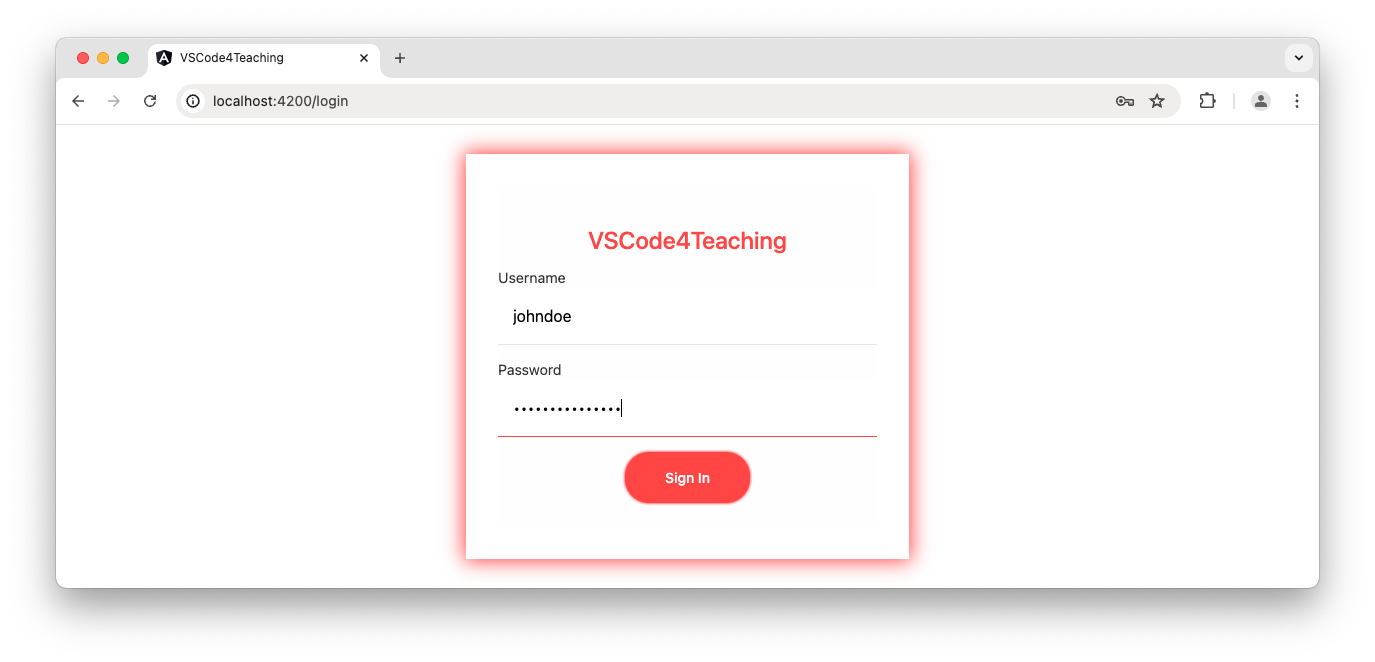
\includegraphics[width=\textwidth]{imagenes/utilizadas/4-3-implementacion/rf1-1.png}
    \caption{Formulario de inicio de sesión para usuarios registrados en la aplicación web.}
    \label{fig:reqf1-1}
\end{figure}

Una vez cumplimentado, las credenciales se envían al servidor y, en caso de ratificarse su validez, se genera un \textit{token} relativo a la sesión activa del usuario que queda almacenado en el contexto de la pestaña activa mediante el uso del \textit{sessionStorage}, que es un almacenamiento del navegador que permite almacenar pares clave-valor que persisten únicamente al contexto de la página que los crea (por contraposición con el \textit{localStorage}, que persiste a la finalización de la sesión activa salvo que se cierre la sesión ex profeso).

Por otro lado, el requisito \texttt{RF-1.2} especifica que los usuarios autenticados deben poder visualizar los recursos que tenga asociados a su cuenta. Para ello, una vez que los usuarios inician sesión en la aplicación, visualizan una pantalla de inicio que muestra los cursos de los que forman parte (\referenciaFigura{fig:reqf1-2}) que varía según el rol: mientras que los estudiantes tienen un botón para acceder a la pantalla en la que comienzan a realizar ejercicios (\referenciaConTT{subsec:rf9}{RF-9}), los docentes acceden a una interfaz (\referenciaFigura{fig:reqf1-3}) en la que pueden visualizar los ejercicios de los que dispone el curso con información básica sobre el progreso de cada uno y, además, crear nuevos ejercicios (\referenciaConTT{subsec:rf2}{RF-2}), gestionar los alumnos matriculados (\referenciaConTT{subsec:rf6}{RF-6}) y compartir el curso (\referenciaConTT{subsec:rf7}{RF-7}).

\begin{figure}[ht]
    \centering
    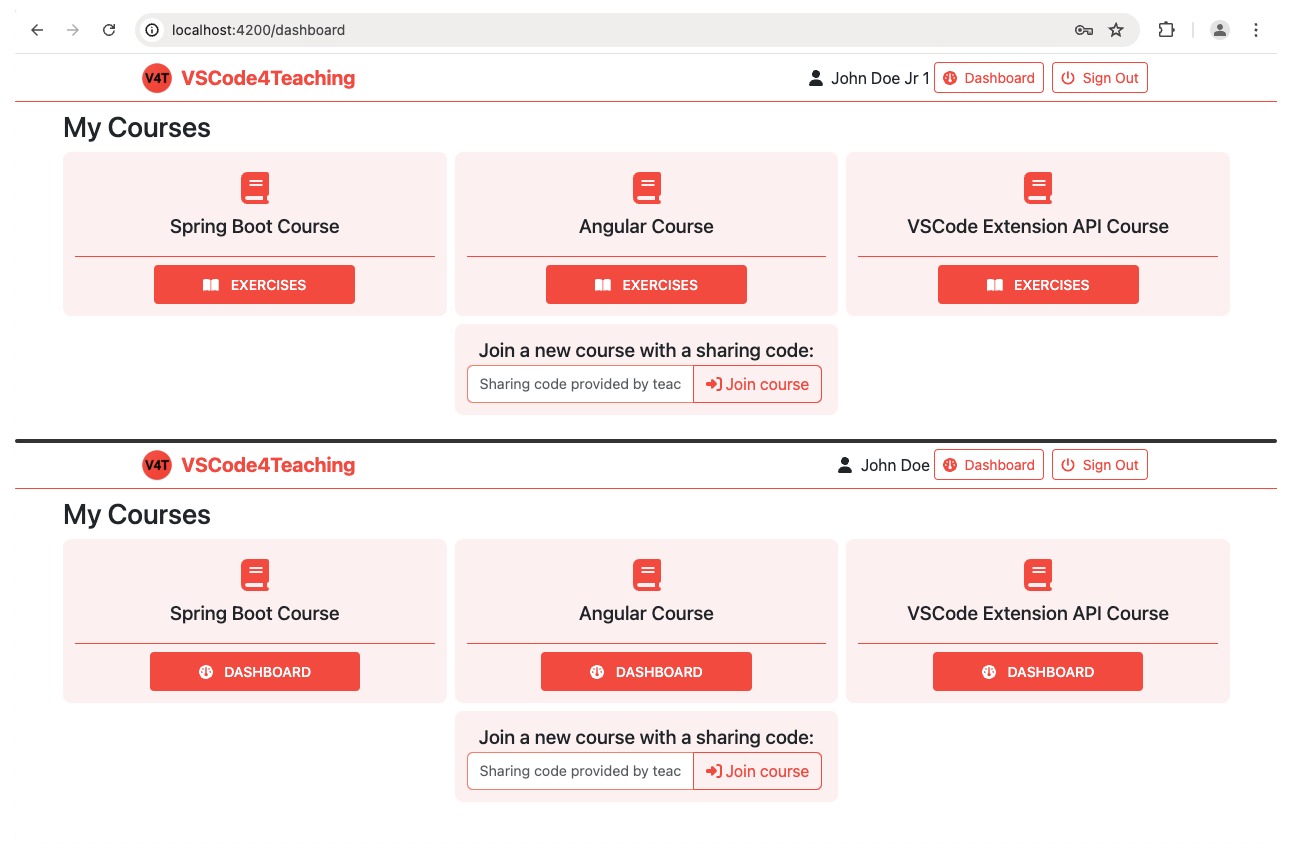
\includegraphics[width=\textwidth]{imagenes/utilizadas/4-3-implementacion/rf1-2.png}
    \caption{Pantalla de inicio para usuarios autenticados, tanto estudiantes (arriba) como docentes (abajo).}
    \label{fig:reqf1-2}
\end{figure}

\begin{figure}[ht]
    \centering
    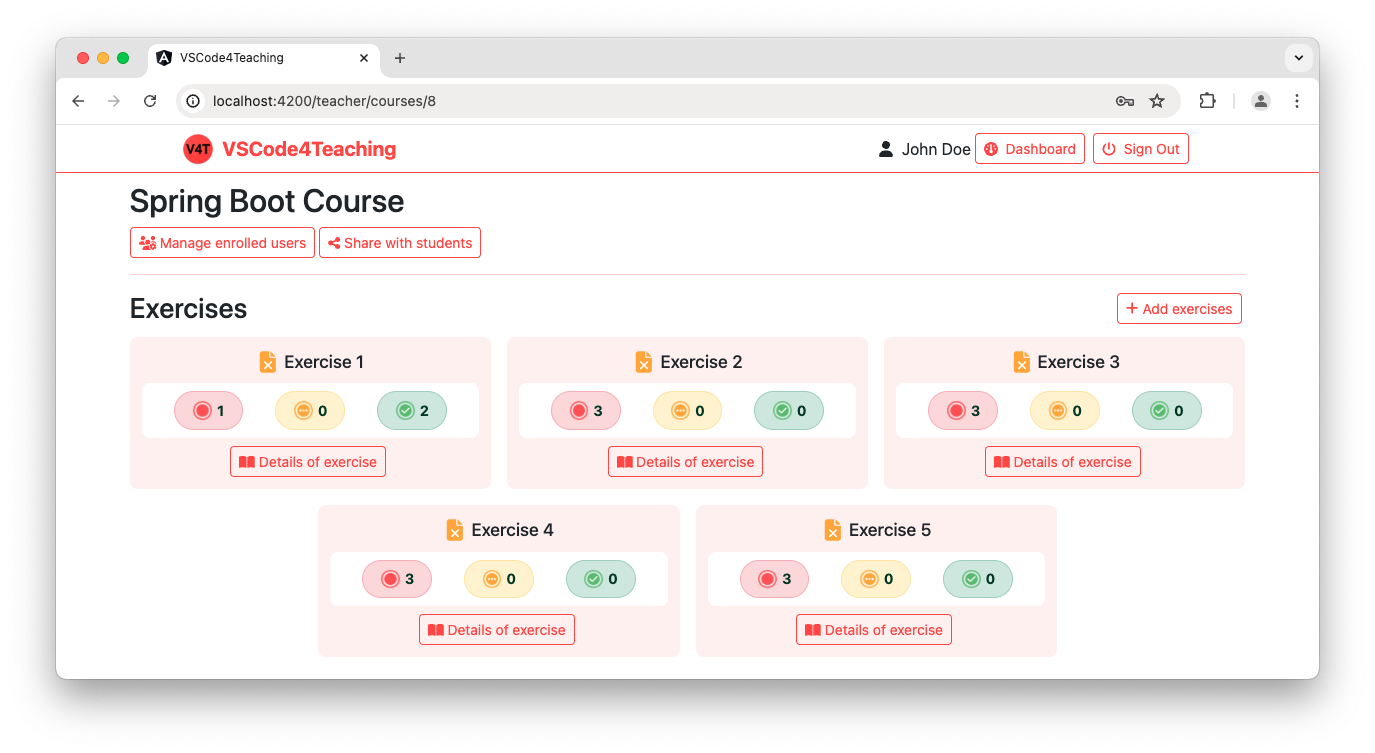
\includegraphics[width=\textwidth]{imagenes/utilizadas/4-3-implementacion/rf1-3.png}
    \caption{Interfaz principal para docentes acerca de cada uno de sus cursos impartidos.}
    \label{fig:reqf1-3}
\end{figure}

\subsubsection{\texttt{RF-2}: creación de nuevos ejercicios}
\label{subsec:rf2}

Los docentes tienen la capacidad de añadir ejercicios nuevos en los cursos que imparten. En la extensión, disponen de sendos botones para añadir un solo ejercicio o varios contenidos en un mismo directorio. Para replicar este comportamiento en la aplicación web, en la pantalla que les permite visualizar el detalle de sus cursos (introducida en el \referenciaConTT{subsec:rf1}{RF-1.2}) disponen de un botón ``Add exercises'' (añadir ejercicios) que despliega un modal con todos los elementos y controles necesarios para poder crear nuevos ejercicios.

En un primer momento, el modal solicita al profesor que seleccione un directorio disponible en su sistema local de ficheros. Una vez elegido el directorio, el navegador solicitará permiso de lectura de sus contenidos a través de la \textit{File System Access API} (véase la \referenciaSeccion{subsec:tecFSA}) y, una vez concedido, se determinará automáticamente si el directorio contiene únicamente la plantilla o si tiene, además, propuesta de solución del docente. Se considera que un ejercicio dispone de plantilla de solución si su directorio raíz contiene, al menos, dos directorios \textit{template} y \textit{solution} cuyos contenidos serán tomados, respectivamente, como la plantilla y la propuesta de solución ---formato ya empleado anteriormente en la extensión---; interpretándose en otro caso que todos los contenidos conforman la plantilla. Esta exploración puede realizarse directamente en el directorio elegido o en cada subdirectorio que contenga, considerando cada uno de ellos como un nuevo ejercicio y determinando en cada caso si tienen propuesta de solución o únicamente plantilla.

\begin{figure}[ht]
    \centering
    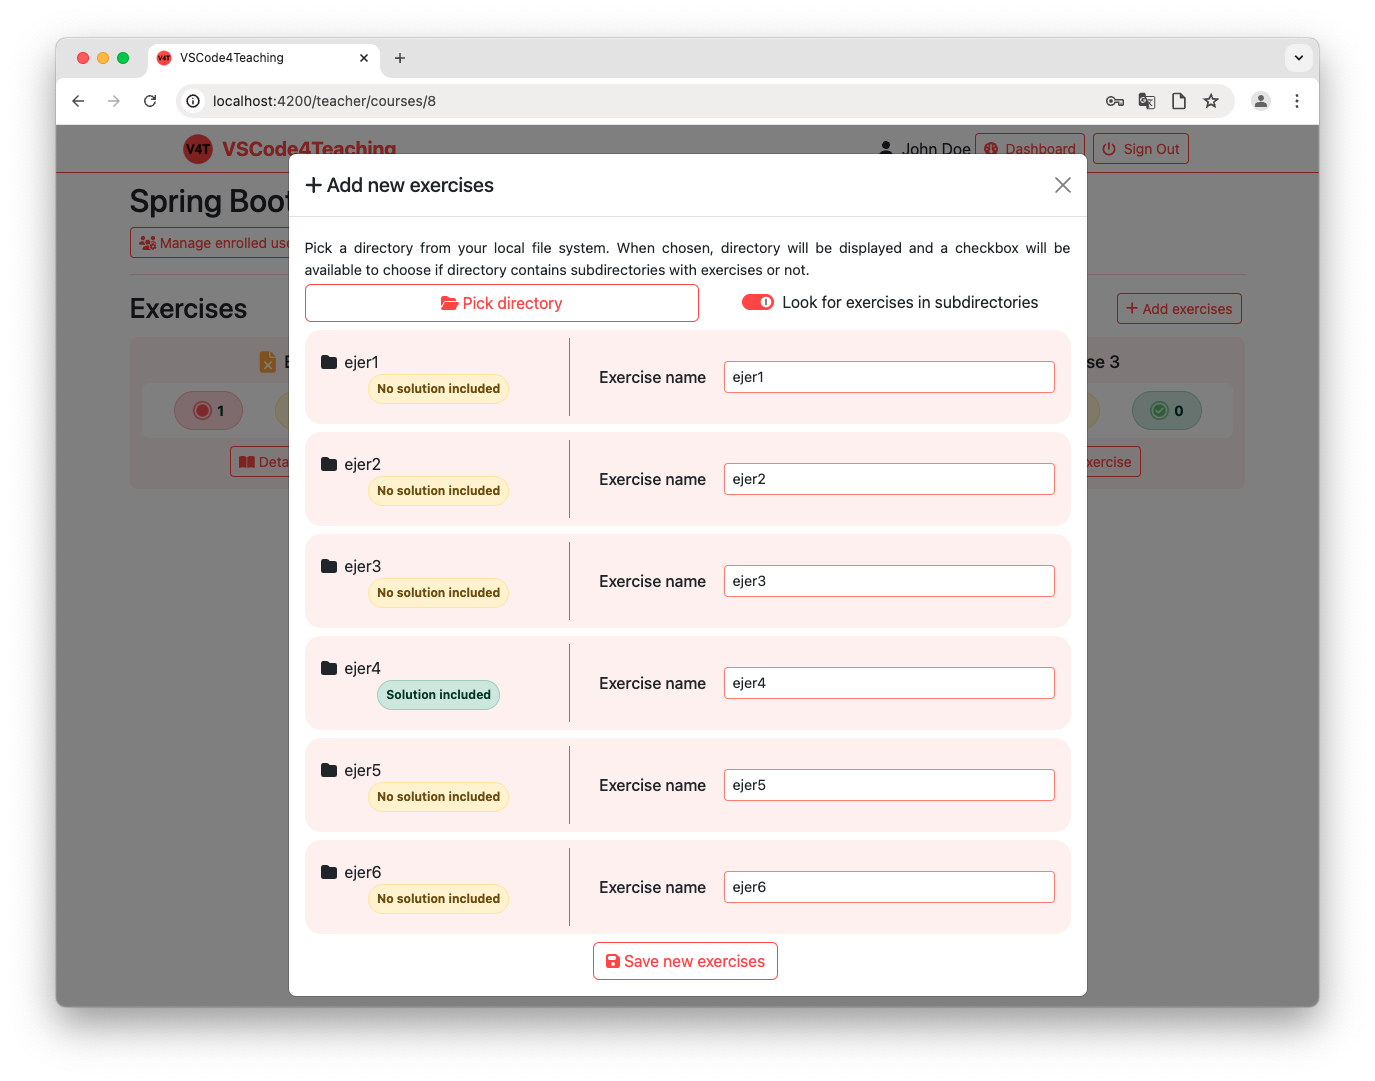
\includegraphics[width=\textwidth]{imagenes/utilizadas/4-3-implementacion/rf2-1.png}
    \caption{Ventana modal para la creación de nuevos ejercicios tras analizar los contenidos del directorio elegido.}
    \label{fig:reqf2-1}
\end{figure}

Una vez elegido un directorio y determinado si se desea emplear directamente esta carpeta o sus contenidas, se muestra una lista con los ejercicios reconocidos, mostrando para cada uno el directorio local del que proceden y un campo que permite configurar su nombre, tomando por defecto el nombre del directorio que contiene los ficheros asociados. Se muestra un ejemplo en la \referenciaFigura{fig:reqf2-1}, en la que se escoge revisar las carpetas contenidas en el directorio elegido, observando que únicamente una de ellas contiene una propuesta de resolución.

Cuando se han determinado los nombres para los ejercicios, es posible iniciar su creación. Este proceso, para cada ejercicio, ejecuta una primera petición para generar el ejercicio en el servidor y, cuando obtiene respuesta, se comprimen en el navegador los ficheros que conforman la plantilla, enviándola una vez comprimida en una nueva petición. En caso de incluir propuesta de solución, a este proceso se suma una nueva compresión y petición para guardar la propuesta de solución. Se ejecutan todos los procesos para la creación de ejercicios concurrentemente, tal como evidencia la \referenciaFigura{fig:reqf2-2}, informando a través de una barra de progreso e indicadores de estado del avance del proceso para cada ejercicio. Solo cuando hayan terminado todos los procesos, el modal podrá ser cerrado.

\begin{figure}[ht]
    \centering
    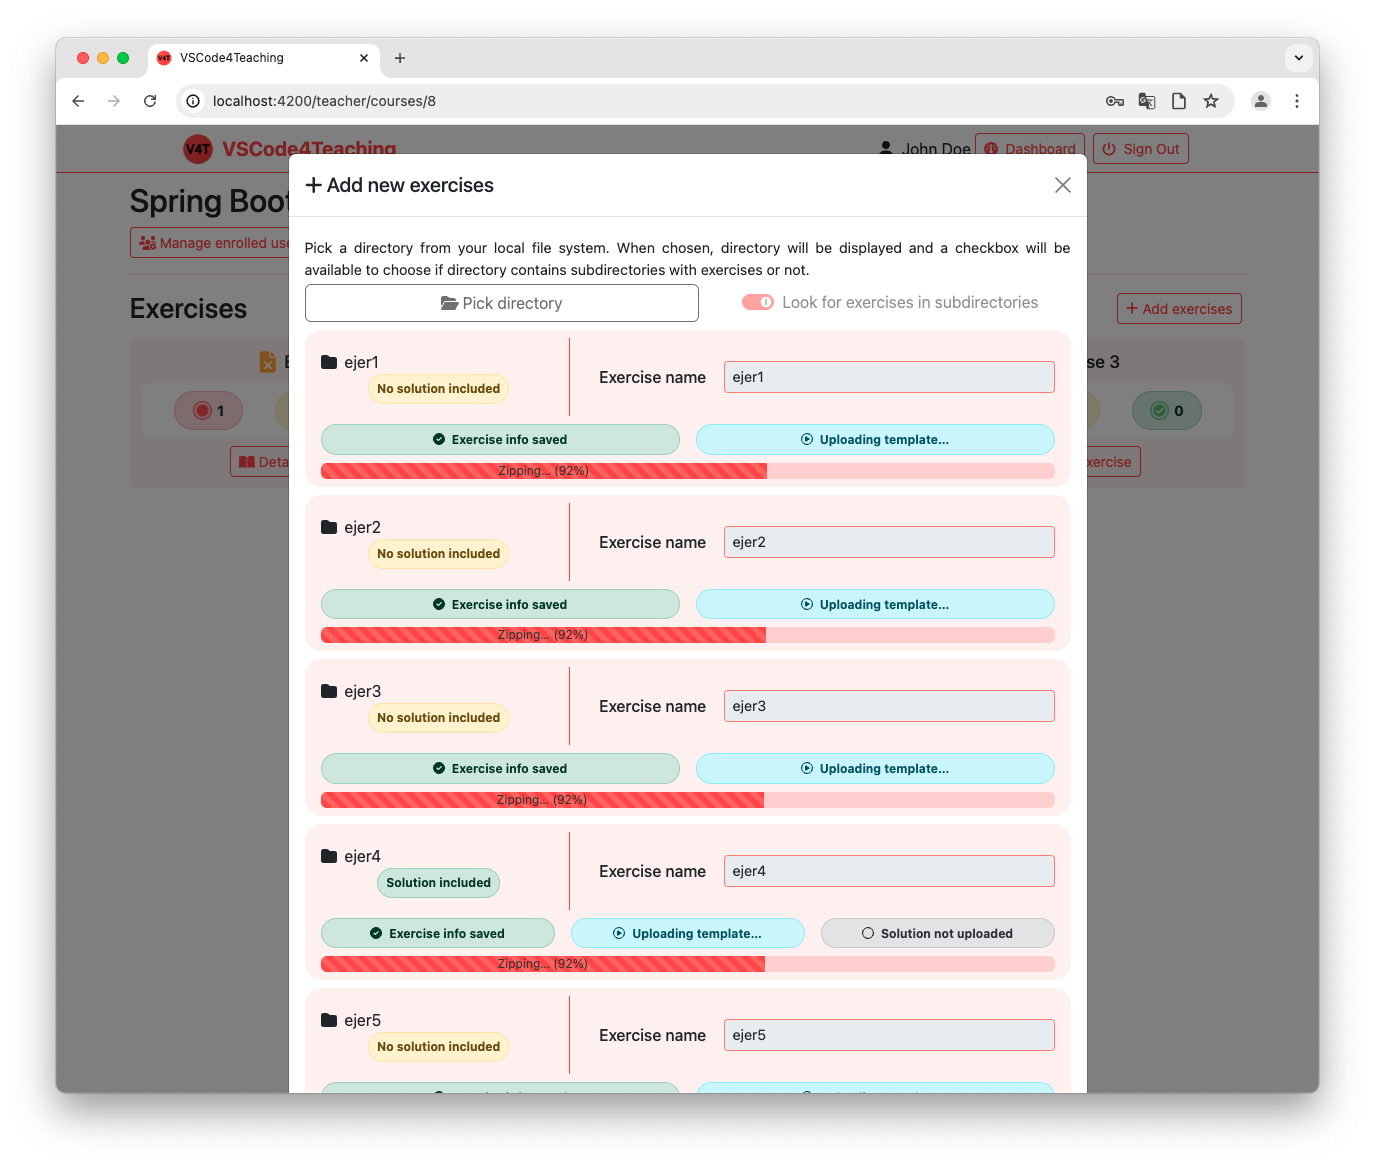
\includegraphics[width=\textwidth]{imagenes/utilizadas/4-3-implementacion/rf2-2.png}
    \caption{Instantánea de la ejecución del proceso de creación de nuevos ejercicios.}
    \label{fig:reqf2-2}
\end{figure}

\subsubsection{\texttt{RF-3}: seguimiento en tiempo real de progreso de ejercicios}
\label{subsec:rf3}

Cuando utilizan la extensión para Visual Studio Code, los docentes disponen de la capacidad para visualizar el \textit{dashboard} de un ejercicio, que muestra métricas actualizadas en tiempo real sobre el progreso de los estudiantes. Del mismo modo, la extensión incorpora una pantalla muy parecida que permite realizar un seguimiento en tiempo real sobre cada ejercicio de los cursos impartidos por un docente.

\begin{figure}[ht]
    \centering
    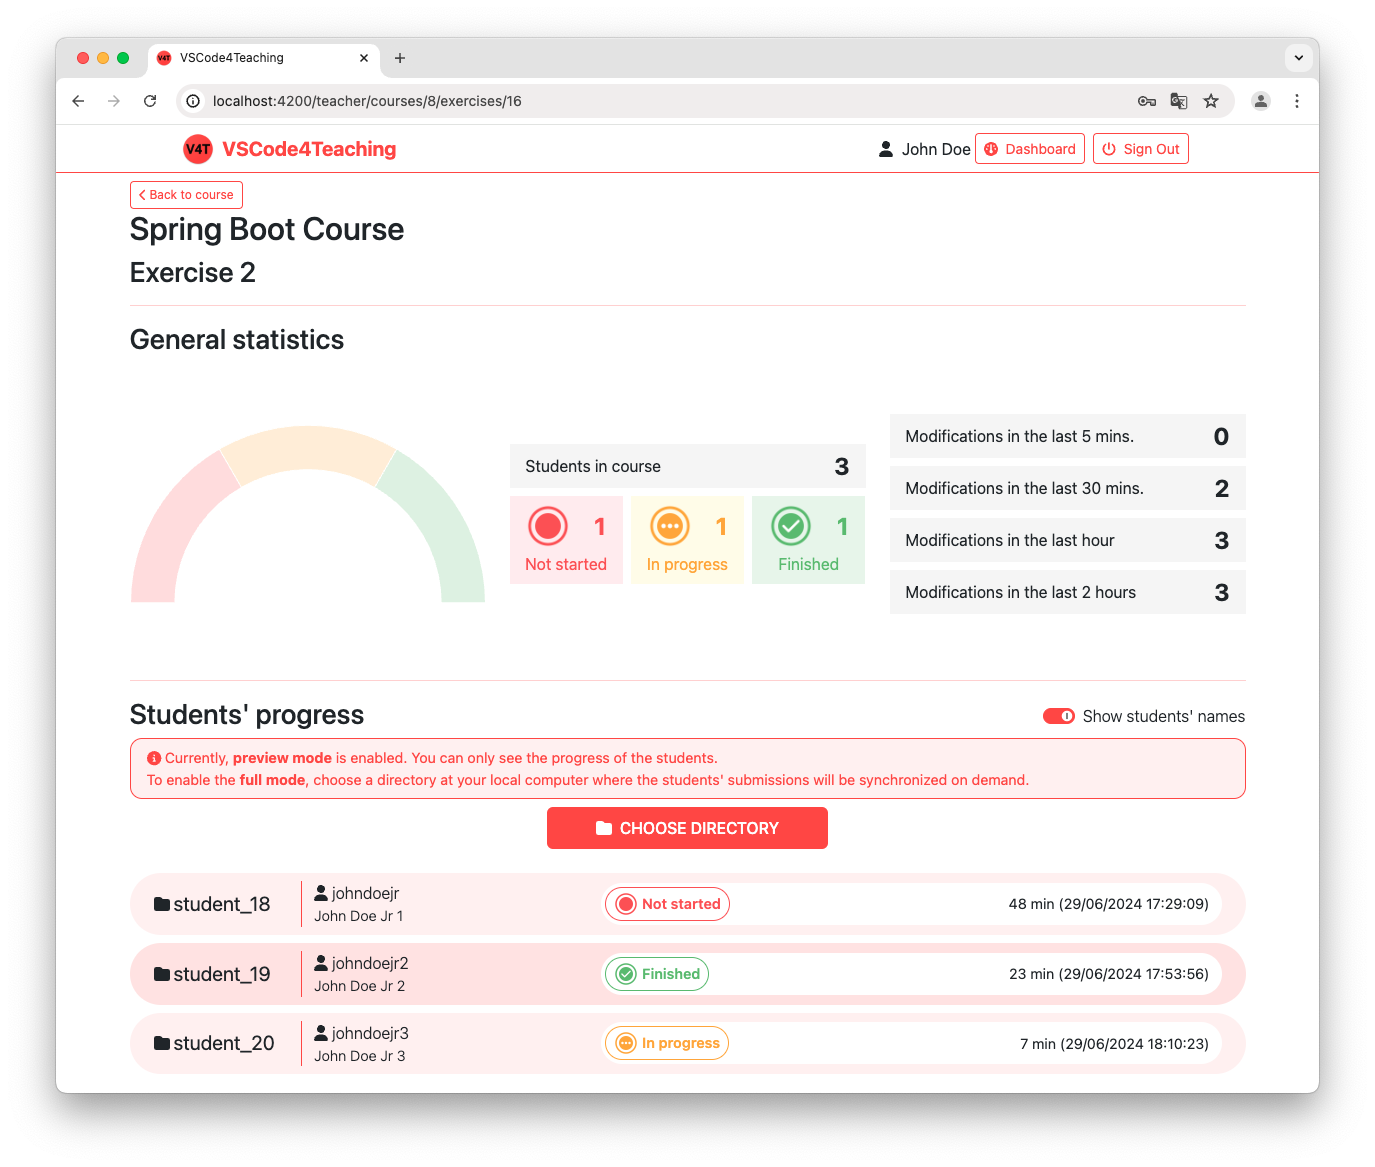
\includegraphics[width=\textwidth]{imagenes/utilizadas/4-3-implementacion/rf3-1.png}
    \caption{\textit{Dashboard} de un ejercicio en la aplicación web con métricas actualizadas en tiempo real para el seguimiento del progreso de los estudiantes.}
    \label{fig:reqf3-1}
\end{figure}

Se incluye una captura de esta visualización en la \referenciaFigura{fig:reqf3-1}. Esta visualización permite ver a los docentes rápidamente cuántos estudiantes hay matriculados en el curso ---y, por tanto, cuántos alumnos realizarán potencialmente el ejercicio---, desgranados debajo según el progreso, diferenciando los que no lo han iniciado, los que están realizándolo y los que lo han finalizado, incluyendo una gráfica semicircular representativa adyacente. Además, también se muestra cuántos estudiantes han modificado su propuesta en los últimos cinco y treinta minutos, en la última hora y dos horas. Debajo de estas estadísticas generales, es posible visualizar el progreso individualizado de cada estudiante, que se muestra de forma anónima: junto a cada directorio de cada propuesta de resolución aparecen el estado del ejercicio y la fecha y tiempo transcurrido tras la última modificación. Es posible asociar cada propuesta de resolución a su autor al modificar el control ``Show students' names'', lo que hará que se muestre en cada fila, además, el apodo y nombre completo de cada estudiante.

La extensión permite disponer del \textit{dashboard} en dos formatos: en forma de previsualización, mostrando únicamente las métricas anteriormente relatadas, o en formato completo, permitiendo abrir los ficheros que componen la propuesta de cada estudiante. Análogamente, la aplicación web permite visualizar únicamente las métricas en formato de previsualización y, además, da al docente la opción de escoger un directorio local para descargar en él bajo demanda las distintas propuestas de los estudiantes, tal como se detalla en el requisito \referenciaConTT{subsec:rf4}{RF-4}.

\subsubsection{\texttt{RF-4}: obtención bajo demanda de ficheros de ejercicios}
\label{subsec:rf4}

\begin{figure}[ht!]
    \centering
    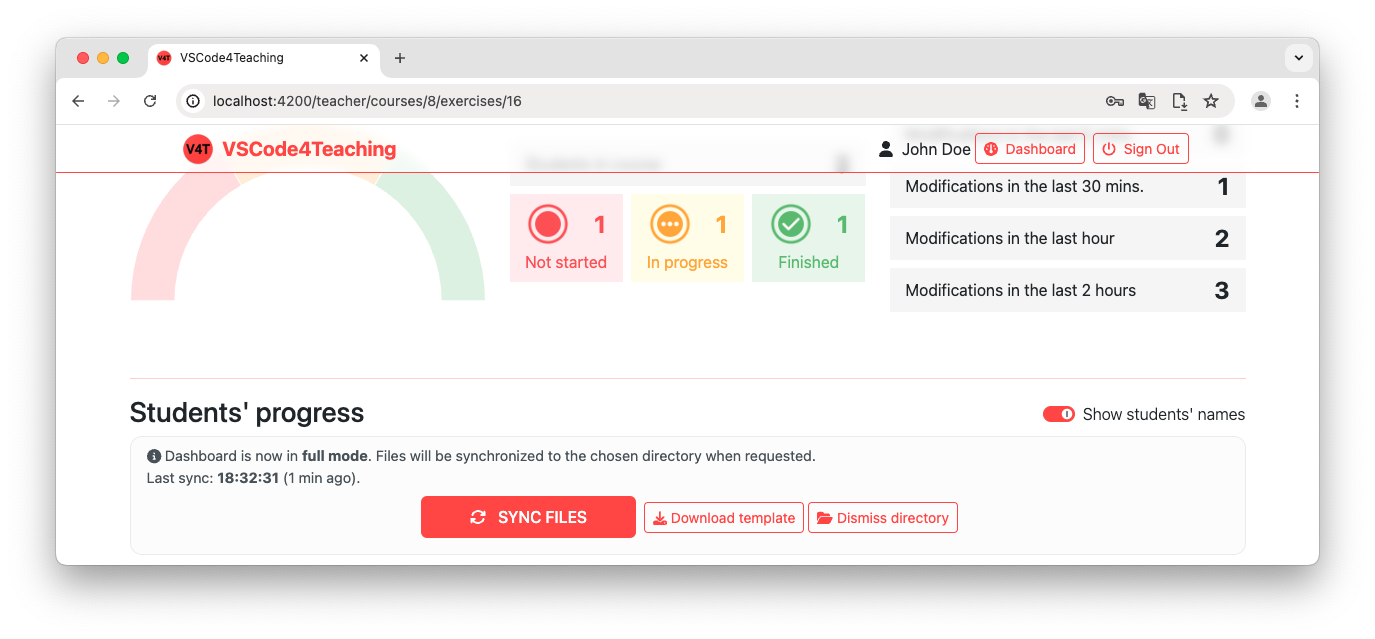
\includegraphics[width=\textwidth]{imagenes/utilizadas/4-3-implementacion/rf4-1.png}
    \caption{Fragmento del \textit{dashboard} que informa sobre la descarga de los ficheros de las propuestas de resolución de los estudiantes.}
    \label{fig:reqf4-1}
\end{figure}

El \textit{dashboard} de cada ejercicio disponible en la extensión permite, en su formato completo, abrir los ficheros que conforman la propuesta de resolución de cada estudiante y, además, visualizar gráficamente en Visual Studio Code las diferencias existentes entre las propuestas y la plantilla original. Análogamente, y dentro de las capacidades que permiten las tecnologías empleadas (descritas en la \referenciaSeccion{subsec:tecAppWeb}), la aplicación web brinda a los docentes la capacidad de descargar bajo demanda todas las propuestas de resolución para poder visualizarlas en local en el editor de su preferencia.

El requisito \referenciaConTT{subsec:rf3}{RF-3} introduce el funcionamiento y las capacidades de las que dispone el \textit{dashboard} de ejercicios implementado en la aplicación web. En la sección acerca del progreso de los estudiantes, tal como se puede apreciar en la \referenciaFigura{fig:reqf3-1}, se dispone un botón ``Choose directory'' (elegir directorio) que permite a los docentes escoger una carpeta en su máquina sobre la que concederán permisos de lectura y escritura para descargar en ella las propuestas de resolución de los estudiantes bajo demanda.

Tal como refleja la \referenciaFigura{fig:reqf4-1}, al escoger una carpeta local se habilitan nuevas opciones para los docentes, análogas al ``modo completo'' del \textit{dashboard} de la extensión, permitiendo la sincronización de los ficheros de los estudiantes bajo demanda, registrando cuándo fueron descargados por última vez. Esta sincronización es unidireccional, ya que no se registran las modificaciones locales realizadas por los docentes y, además, la descarga sobrescribe los ficheros previamente existentes en local. Se permite al profesor, adicionalmente, descargar la plantilla del ejercicio (y la propuesta de solución si la tuviera) en el mismo directorio.

\subsubsection{\texttt{RF-5}: configuración de publicación de solución de ejercicios}
\label{subsec:rf5}

\begin{figure}[!ht]
    \centering
    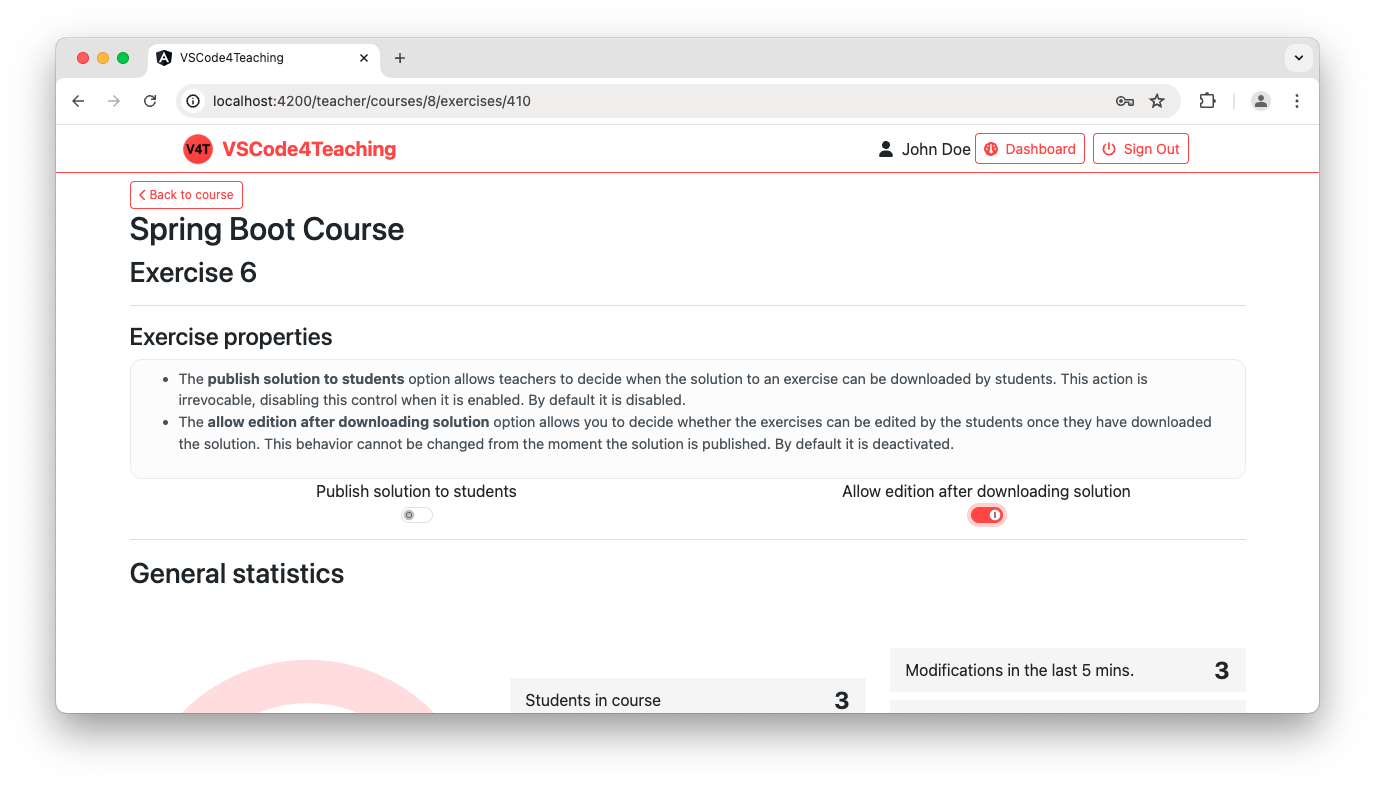
\includegraphics[width=0.9\textwidth]{imagenes/utilizadas/4-3-implementacion/rf5-1.png}
    \caption{Sección del \textit{dashboard} de los ejercicios que permite configurar los parámetros para la configuración de la disponibilidad y comportamiento de la descarga de la propuesta de solución del docente.}
    \label{fig:reqf5-1}
\end{figure}

Tal como se especifica en el requisito \referenciaConTT{subsec:rf2}{RF-2}, los ejercicios que los docentes añaden en sus cursos pueden tener asociada una propuesta de solución que los estudiantes pueden descargar en la extensión según dos parámetros de configuración de la disponibilidad de la solución que los docentes pueden ajustar en el \textit{dashboard} de cada ejercicio, tal como muestra la \referenciaFigura{fig:reqf5-1}. Los parámetros son:
\begin{itemize}
    \item \textit{Allow edition after downloading solution} (permitir edición tras descargar solución). Permite ajustar si los estudiantes pueden modificar sus propias propuestas tras descargar la solución o si, por el contrario, al descargar la propuesta de solución se deben impedir nuevas ediciones, marcándolo previamente como finalizado. Este parámetro se puede modificar mientras la solución no sea pública.
    \item \textit{Publish solution to students} (publicar solución a estudiantes). Permite configurar la disponibilidad para la descarga de la solución a los estudiantes, quienes dispondrán de un elemento gráfico en la extensión que les permitirá descargar la solución en local para, además, poder compararla mediante una interfaz gráfica para visualizar las diferencias existentes entre su propia propuesta y la solución del docente. La activación de la publicación impide la edición del parámetro anterior y, una vez publicada, esta configuración ya no puede revertirse.
\end{itemize}

\subsubsection{\texttt{RF-6}: gestión de matriculación de usuarios en cursos}
\label{subsec:rf6}

Cuando utilizan la extensión para Visual Studio Code, los docentes tienen la posibilidad de inscribir y eliminar estudiantes y otros profesores de sus cursos. Equivalentemente, se añade a la aplicación web la posibilidad de gestionar las matrículas de un curso. Para ello, tal como introduce el requisito \referenciaConTT{subsec:rf1}{RF-1.2}, los docentes disponen de un botón ``Manage enrolled users'' (gestionar usuarios inscritos) que despliega una ventana modal.

Este modal, tal como se muestra en la \referenciaFigura{fig:reqf6-1}, muestra una lista con todos los usuarios inscritos en el curso, diferenciando a los profesores de los estudiantes. A excepción del profesor creador, cada uno de estos usuarios puede ser eliminado del curso haciendo uso del botón dispuesto en cada fila. Adicionalmente, en la parte inferior se muestra un desplegable que contiene todos los usuarios potencialmente matriculables; esto es, a todos los usuarios salvo a aquellos que ya están matriculados. El profesor puede escoger uno de ellos y, mediante el botón adyacente, inscribirlo en el curso.

\begin{figure}[ht]
    \centering
    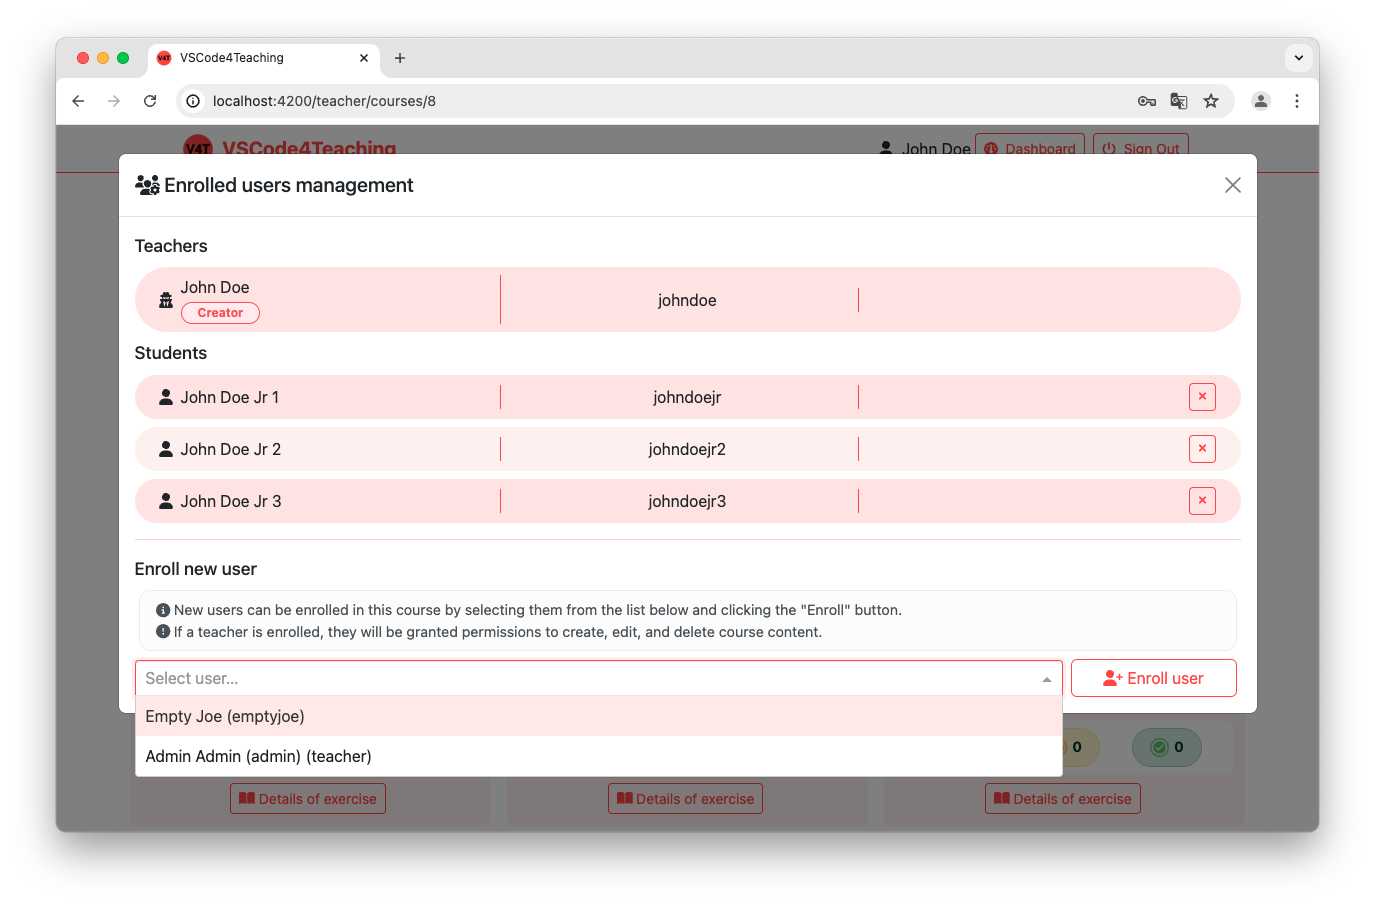
\includegraphics[width=\textwidth]{imagenes/utilizadas/4-3-implementacion/rf6-1.png}
    \caption{Visualización de la lista de usuarios inscritos a un curso y de las capacidades para añadir nuevos usuarios o revocar inscripciones.}
    \label{fig:reqf6-1}
\end{figure}

\subsubsection{\texttt{RF-7}: compartición de código asociado a un curso}
\label{subsec:rf7}

Existen dos formas para hacer que un estudiante quede matriculado en un curso, tanto en la extensión como en la aplicación web: puede ser inscrito manualmente por un profesor (\referenciaConTT{subsec:rf6}{RF-6}) o puede automatricularse (\referenciaConTT{subsec:rf8}{RF-8}), que requiere de un código que deben ser proporcionado por el docente.

La extensión permite a los docentes obtener un enlace al servidor de \textit{VSCode4Teaching} en uso que puede divulgar al estudiantado que desee que se automatricule. Este enlace incluye un código único que identifica biunívocamente cada curso existente en la plataforma. Para generarlo, la visualización de los cursos para docentes (\referenciaConTT{subsec:rf1}{RF-1.2}) dispone de un botón ``Share with students'' (compartir con estudiantes) que, tal como queda plasmado en la \referenciaFigura{fig:reqf7-1}, muestra a los docentes el código único para la automatrícula en el curso como, además, el enlace al servidor que los alumnos pueden abrir en el navegador para consultar información adaptada al caso del curso específicamente divulgado, incluyendo instrucciones acerca de cómo inscribirse en el curso compartido.

\begin{figure}[ht]
    \centering
    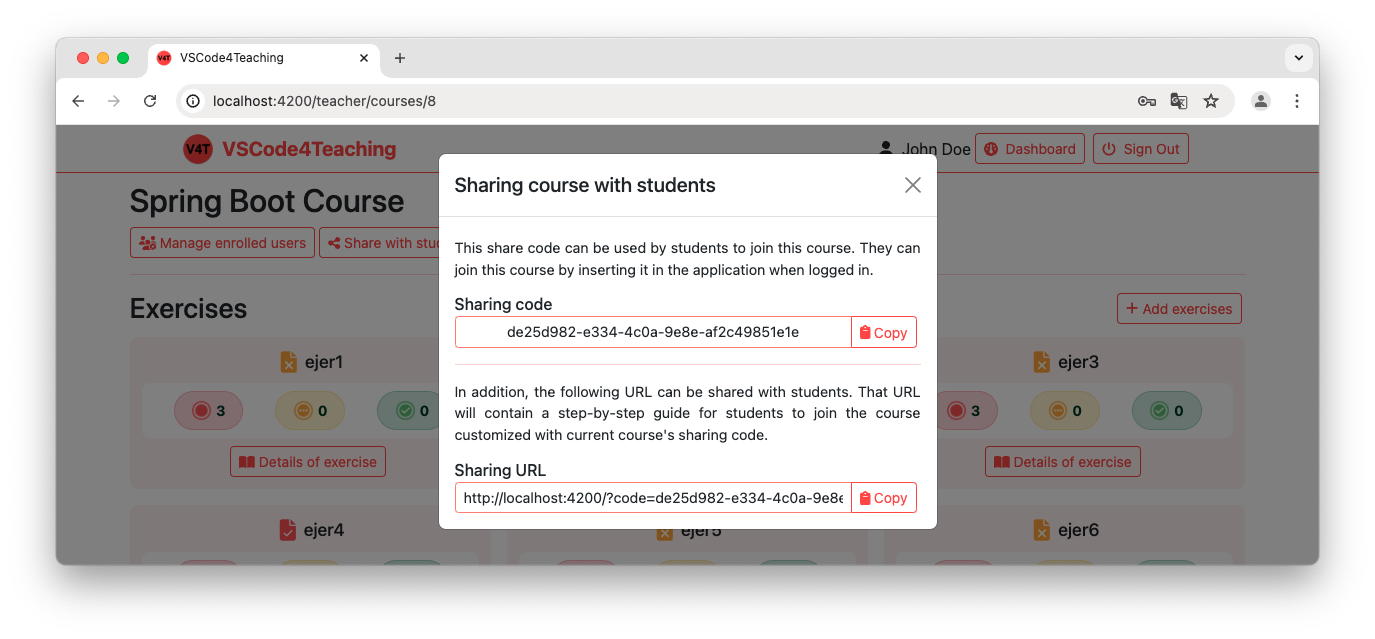
\includegraphics[width=\textwidth]{imagenes/utilizadas/4-3-implementacion/rf7-1.png}
    \caption{Información para la compartición del código único de automatrícula en un curso.}
    \label{fig:reqf7-1}
\end{figure}

\subsubsection{\texttt{RF-8}: automatriculación mediante código de compartición}
\label{subsec:rf8}

Los estudiantes pueden ser matriculados en los cursos manualmente por sus docentes (\referenciaConTT{subsec:rf6}{RF-6}) y, además, tienen la capacidad de inscribirse en cursos por sí mismos utilizando un código proporcionado por sus profesores, ya sea empleando la extensión para Visual Studio Code o a través de la aplicación web. Este requisito es complementario del \referenciaConTT{subsec:rf7}{RF-7}, por el que los docentes disponen de la capacidad para generar códigos de compartición para permitir la autoinscripción de estudiantes en sus cursos.

En caso de querer hacerlo a través de la aplicación web, los estudiantes deben iniciar sesión (\referenciaConTT{subsec:rf1}{RF-1.1}) y, dentro de su página principal, disponen de un campo de texto para introducir el código proporcionado por los docentes, tal como se aprecia en la \referenciaFigura{fig:reqf8-1} y, presionando el botón adyacente, pueden inscribirse en un nuevo curso.

\begin{figure}[ht]
    \centering
    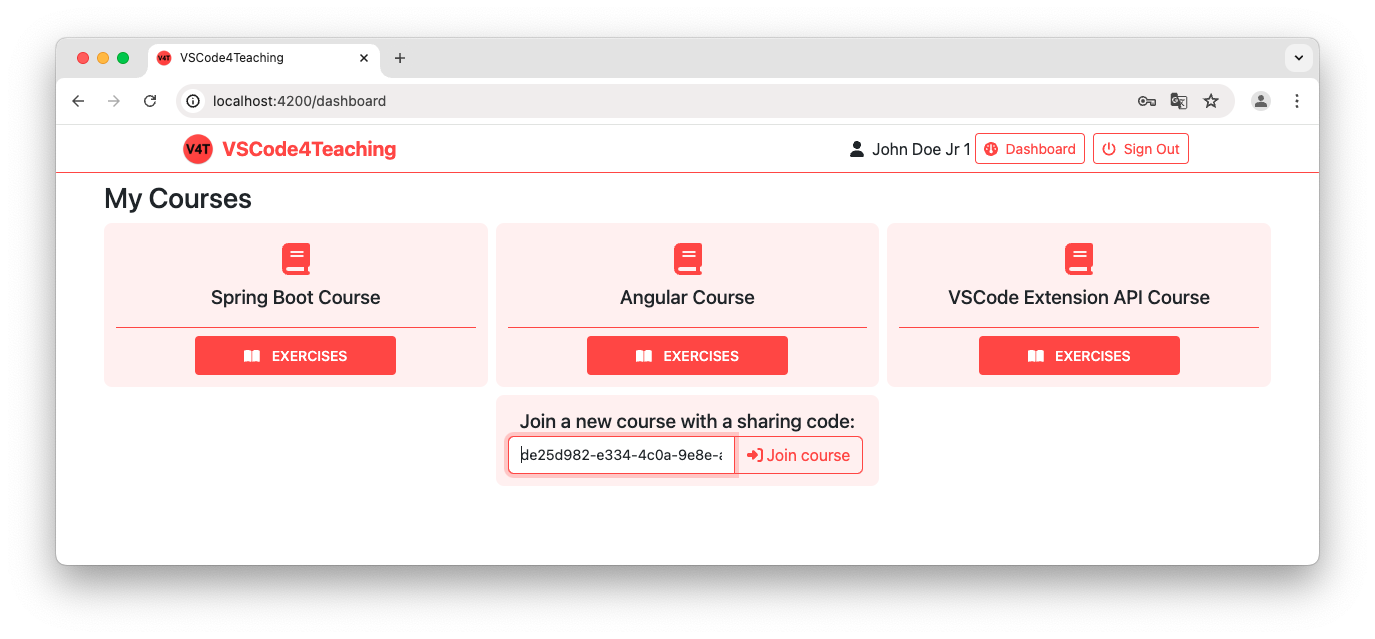
\includegraphics[width=\textwidth]{imagenes/utilizadas/4-3-implementacion/rf8-1.png}
    \caption{Página principal de los estudiantes en la aplicación web con un código de inscripción automática en un curso.}
    \label{fig:reqf8-1}
\end{figure}

\subsubsection{\texttt{RF-9}: visualización de un curso y sus ejercicios}
\label{subsec:rf9}

Una vez autenticados en \textit{VSCode4Teaching} (\referenciaConTT{subsec:rf1}{RF-1.1}), los estudiantes visualizan una pantalla principal o \textit{dashboard} en el que se muestran los cursos en los que están matriculados, tal como se desarrolla en el requisito \referenciaConTT{subsec:rf1}{RF-1.2}. En esta pantalla disponen de un botón ``Exercises'' (ejercicios) en cada curso que les permite acceder al detalle de los ejercicios de cada curso.

Cuando los estudiantes acceden a la visualización del detalle de un curso, la aplicación les solicita primeramente que escojan un directorio del sistema de ficheros de su computador local para alojar los contenidos de los ejercicios del curso, situación inicial que queda reflejada en la \referenciaFigura{fig:reqf9-1}. Si el estudiante ya realizó algún ejercicio, sea total o parcialmente, y mantuvo intacto el directorio que empleó ---esto es, respetando el formato de subdirectorios empleado en local por \textit{VSCode4Teaching}---, puede utilizar la misma carpeta para continuar trabajando, ya que coincidirá el estado de los ejercicios almacenados en local con el progreso sincronizado en el servidor y no se producirán desfases.

\begin{figure}[ht]
    \centering
    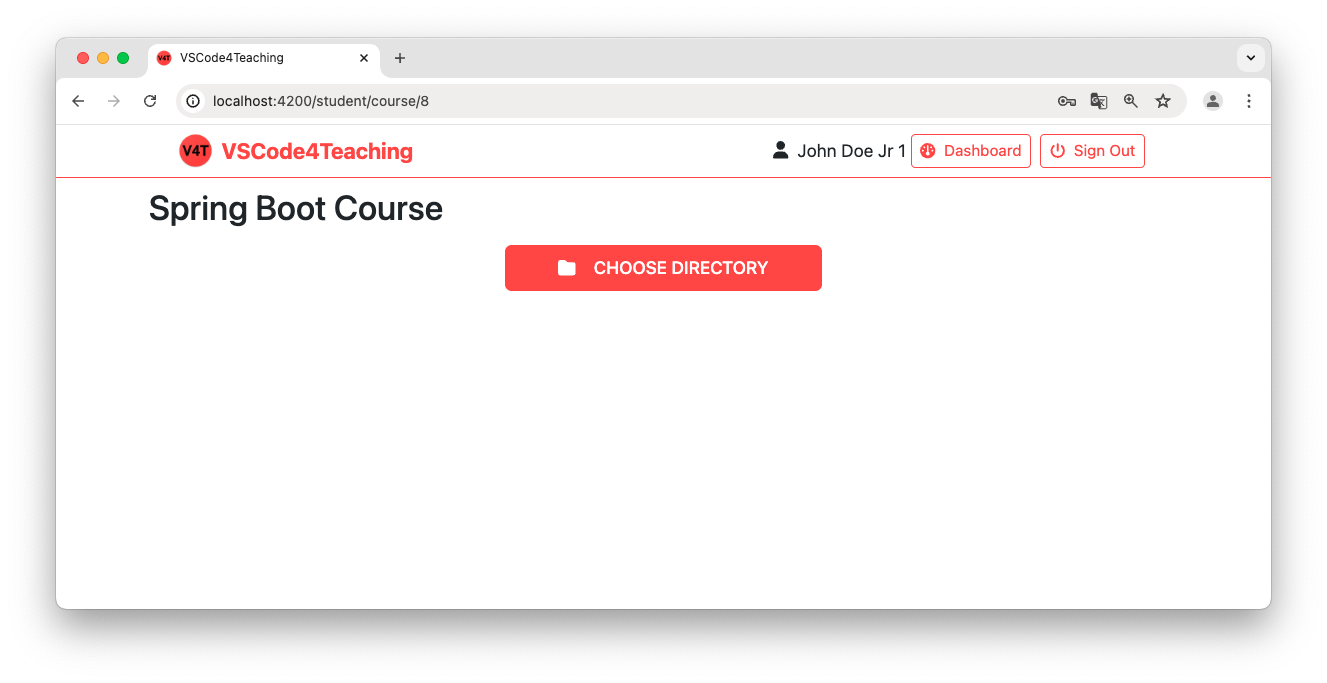
\includegraphics[width=\textwidth]{imagenes/utilizadas/4-3-implementacion/rf9-1.png}
    \caption{Situación inicial de los estudiantes al acceder al detalle de un curso y antes de elegir un directorio local.}
    \label{fig:reqf9-1}
\end{figure}

Una vez escogido el directorio, se muestra a los estudiantes el detalle de los ejercicios asociados al curso, sepárandolos en distintos paneles según su estado de ejecución: los ejercicios en progreso se sitúan en la parte superior, ubicando debajo los ejercicios no comenzados y los finalizados, tal como se refleja en la \referenciaFigura{fig:reqf9-2}. Esta ilustración permite apreciar que el estudiante tiene dos ejercicios pendientes de comenzar (``Exercise 2'' y ``Exercise 5''), ubicados dentro del panel sombreado en rojo con título ``Not started'' (no comenzado) y, además, ha finalizado un ejercicio (``Exercise 3'') que aparece dentro del panel sombreado en verde con título ``Finished'' (finalizado). A estos se suman dos ejercicios dentro del panel amarillo con título ``In progress'' (en progreso), que el estudiante podrá descargar o empezar a sincronizar, posibilidades implementadas en el requisito \referenciaConTT{subsec:rf10}{RF-10}.

\begin{figure}[ht]
    \centering
    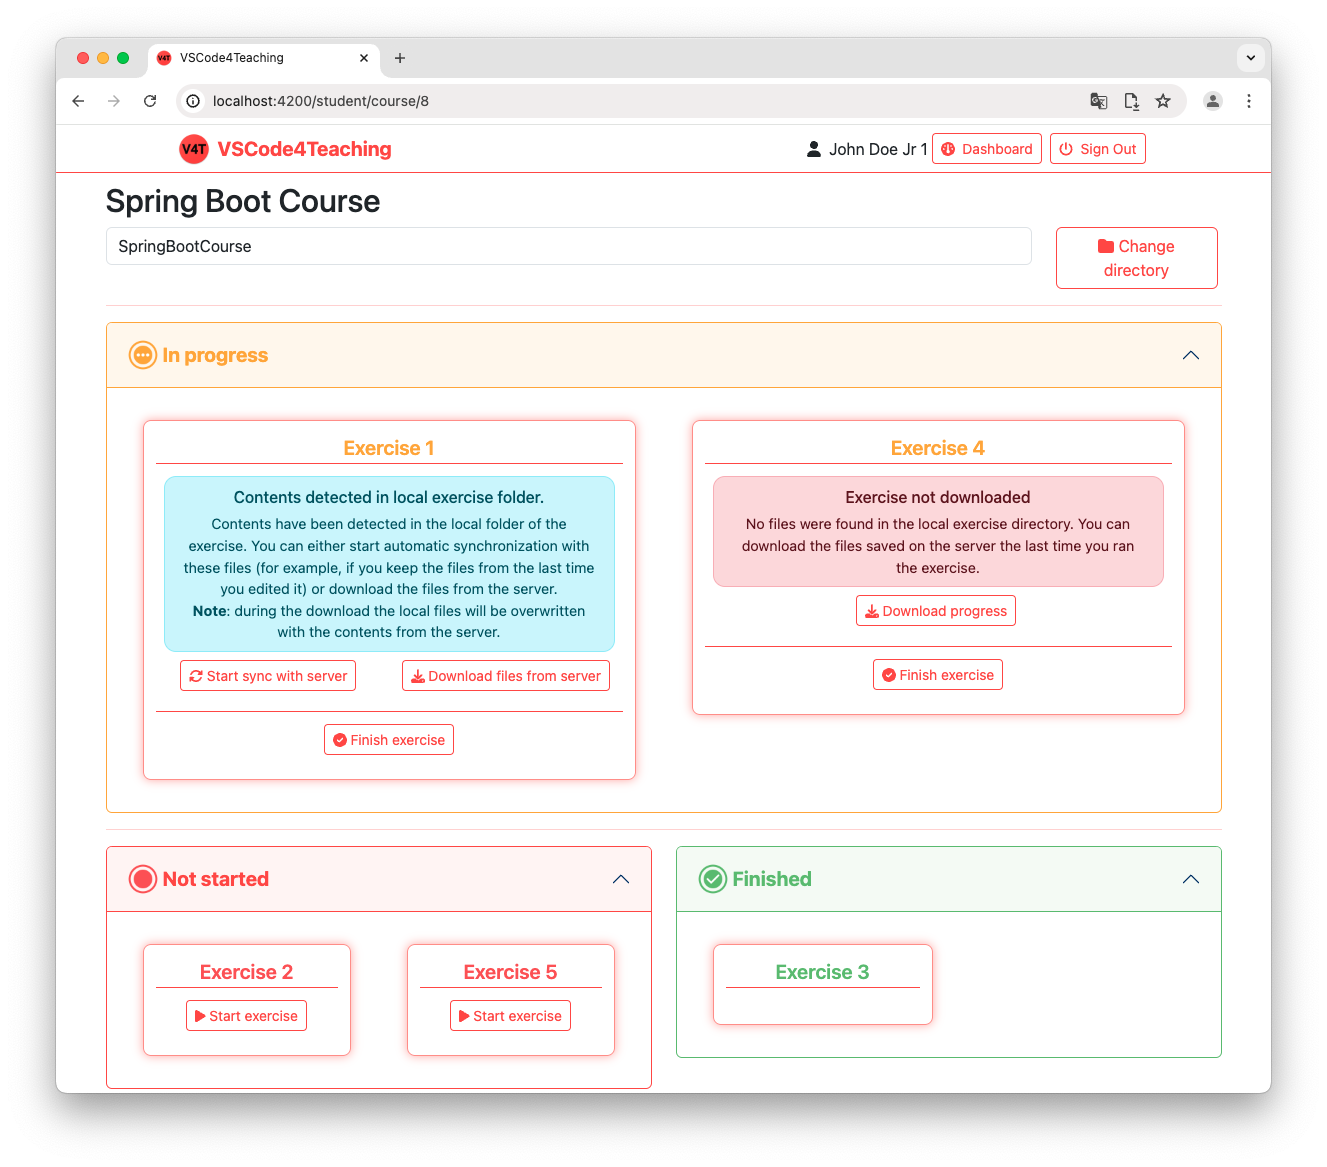
\includegraphics[width=\textwidth]{imagenes/utilizadas/4-3-implementacion/rf9-2.png}
    \caption{Visualización detallada de un curso matriculado por un estudiante con ejercicios ubicados en distintos paneles según su estado.}
    \label{fig:reqf9-2}
\end{figure}

\subsubsection{\texttt{RF-10}: descarga de los ficheros de una propuesta propia de resolución de un ejercicio}
\label{subsec:rf10}

Dentro de la visualización del detalle de un curso matriculado, y tras escoger un directorio local para sincronizar los ficheros, un estudiante puede visualizar todos los ejercicios del curso diferenciados en distintos paneles según su estado de ejecución, tal como especifica el \referenciaConTT{subsec:rf9}{RF-9}.

En el caso de los ejercicios en progreso, al escoger el directorio, la aplicación buscará si existe una versión local del ejercicio, transitando entre los distintos estados reflejados en la \referenciaFigura{fig:reqf10-1}. En caso de no existir ninguna carpeta hija del directorio elegido coincidente con un ejercicio en progreso, la aplicación informará al usuario de que deberá descargar el punto de progreso que haya almacenado en el servidor, tal como ocurre con el ``Exercise 4'' en la \referenciaFigura{fig:reqf9-2}. Si, por el contrario, existe un directorio local que coincida con el ejercicio en progreso, la aplicación pregunta al usuario si desea descargar la versión existente en remoto y sobrescribir los ficheros que colapsen respecto a la versión en local o si, por el contrario, desea iniciar de inmediato la sincronización con el servidor. Este primer escenario es el que sucede en el caso del ``Exercise 1'' de la \referenciaFigura{fig:reqf9-2}.

Estos dos estados iniciales están reflejados en la parte izquierda de la \referenciaFigura{fig:reqf10-1}. Al descargar el ejercicio, se transita al estado que se observa en la parte central de la representación, durante el que la aplicación descarga como fichero comprimido los contenidos del ejercicio proporcionados por el servidor y los descomprime en una carpeta propicia específica dentro del directorio elegido por el estudiante, informando de forma visual a través de dos indicadores del estado activo y una barra de progreso. Una vez preparado el directorio del ejercicio, sea porque ha finalizado la descarga y descompresión o porque se ha iniciado la sincronización de contenidos previamente existentes, se inicia la sincronización automática, reflejada visualmente como muestra la parte derecha de la \referenciaFigura{fig:reqf10-1}. Esta sincronización queda detalladamente explicada en el requisito \referenciaConTT{subsec:rf11}{RF-11}.

\begin{figure}[ht]
    \centering
    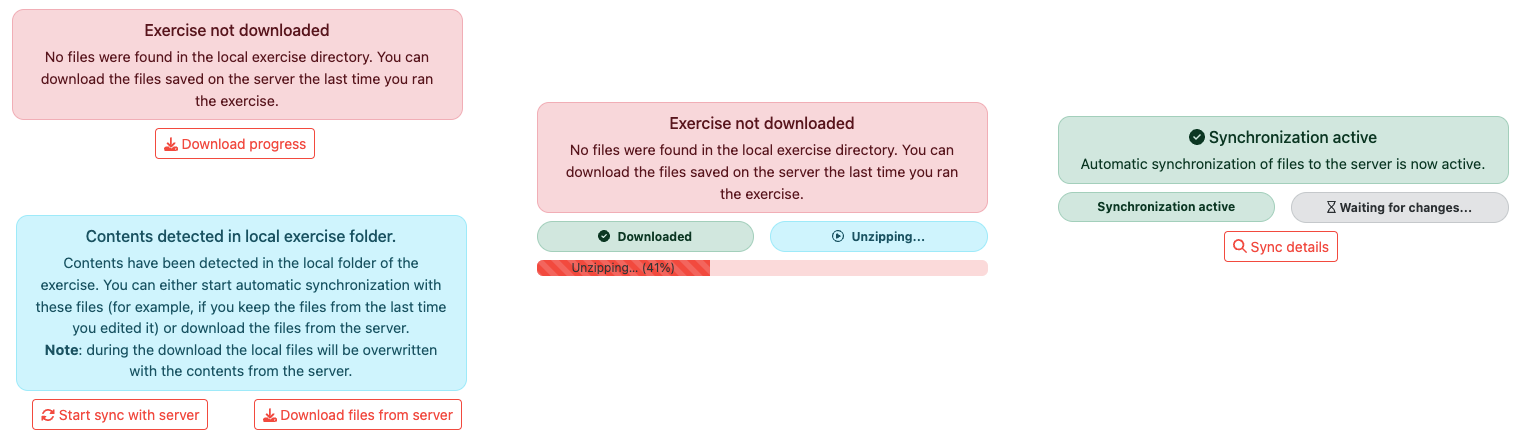
\includegraphics[width=\textwidth]{imagenes/utilizadas/4-3-implementacion/rf10-1.png}
    \caption{Representación de la evolución entre los posibles estados visuales de los ejercicios en progreso según su disponibilidad local.}
    \label{fig:reqf10-1}
\end{figure}

\subsubsection{\texttt{RF-11}: sincronización automática de las modificaciones en los ejercicios durante su realización}
\label{subsec:rf11}

Dentro de la visualización del detalle de los cursos, una vez se ha seleccionado un directorio (\referenciaConTT{subsec:rf9}{RF-9}) y se ha descargado el estado de los ejercicios en progreso o se ha decidido utilizar la información previamente disponible en local (\referenciaConTT{subsec:rf10}{RF-10}), estos ejercicios comienzan a sincronizarse automáticamente con el servidor.

En lo que a la interacción con el usuario respecta, la interfaz muestra para cada ejercicio en progreso dos señales de activación de la sincronización automática y de su estado. La \referenciaFigura{fig:reqf11-1} refleja la visualización de los dos estados posibles: o bien la aplicación se encuentra esperando a que ocurran nuevos cambios y la sincronización del ejercicio está finalizada porque no hay nuevos cambios a comunicar al servidor (izquierda), o bien se está produciendo la transmisión al servidor de las modificaciones de uno o más ficheros (derecha). Los indicadores mostrados en esta figura quedan encuadrados dentro del estado de cada ejercicio.

\begin{figure}[ht]
    \centering
    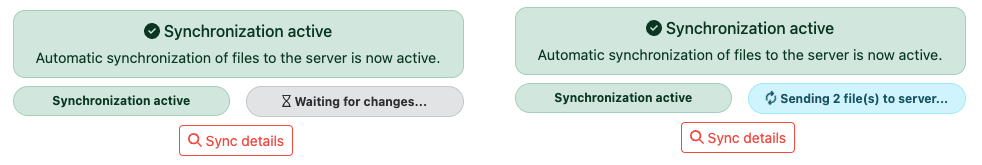
\includegraphics[width=0.9\textwidth]{imagenes/utilizadas/4-3-implementacion/rf11-1.png}
    \caption{Captura de las señales de sincronización activa y estado de la sincronización de ejercicios en progreso.}
    \label{fig:reqf11-1}
\end{figure}

El segundo elemento es el botón ``Sync details'' (detalles de la sincronización) que se muestra debajo del estado de la sincronización en cada ejercicio (visible en la \referenciaFigura{fig:reqf11-1}). Cuando se pulsa, se despliega un modal que contiene una lista con el histórico de los diez ficheros sincronizados más recientemente, los diez siguientes ficheros que serán sincronizados y el que está siendo transmitido al servidor en el momento presente, que dispone de una barra de progreso indicativa del avance de la operación.

La \referenciaFigura{fig:reqf11-2} muestra dos ejemplos de este modal: uno durante la sincronización de un fichero muy pesado (arriba) y otro que refleja la sincronización de una ingente cantidad de ficheros (abajo), constando de una lista de más de 150 ficheros sincronizados y de más de 300 ficheros pendientes de sincronizar. Para cada fichero sincronizado o pendiente de subir, se incluyen dos iconos: uno para reflejar el estado de la subida (rojo si está pendiente, amarillo si está en progreso y verde si se finalizó) y otro que indica el tipo de sincronización, pudiendo tratarse de la creación de un fichero (verde), una modificación de un fichero previamente existente (amarillo) o una eliminación (rojo). Los renombramientos aparecen como eliminaciones y nuevas creaciones.

\begin{figure}[ht]
    \centering
    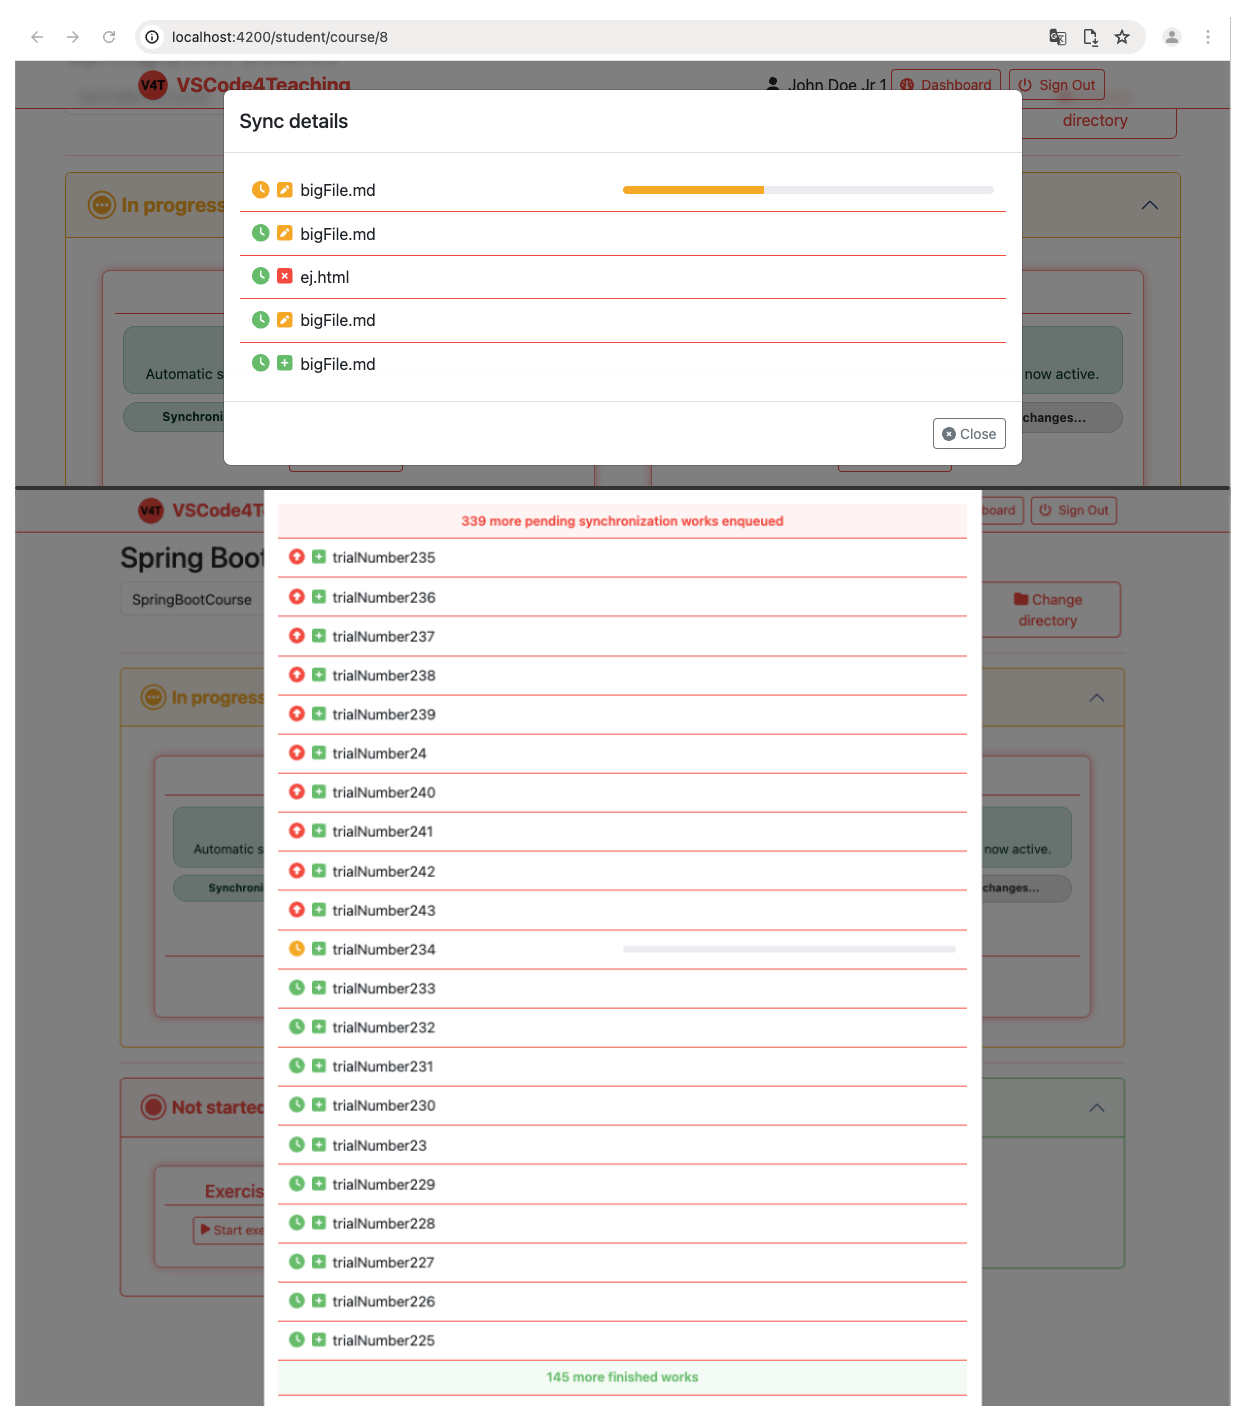
\includegraphics[width=0.8\textwidth]{imagenes/utilizadas/4-3-implementacion/rf11-2.png}
    \caption{Captura del modal explicativo de la sincronización de ficheros de un ejercicio.}
    \label{fig:reqf11-2}
\end{figure}

El diseño e implementación del algoritmo destinado a los procesos automáticos de cotejamiento y sincronización de cada ejercicio en progreso queda desarrollado pormenorizadamente en el \referenciaAnexo{anx:bajoNivelRF11}.

\subsubsection{\texttt{RF-12}: marcado de ejercicio como finalizado}
\label{subsec:rf12}

Tal como introduce el \referenciaConTT{subsec:rf9}{RF-9}, los estudiantes disponen de la capacidad para visualizar el detalle de los cursos en los que están matriculados al seleccionar un directorio local, pudiendo ver los ejercicios que los componen, en qué etapa del progreso de su realización se encuentran y realizar distintas acciones con ellos según su estado: mientras que los no comenzados únicamente pueden ser iniciados y pasan al estado ``en progreso'' (\referenciaConTT{subsec:rf10}{RF-10}), los ejercicios que se están realizando y sincronizando en tiempo real pueden ser finalizados. Para ello, los estudiantes pueden pulsar el botón ``Finish exercise'' (finalizar ejercicio) que aparece en la parte inferior de cada uno de los ejercicios en progreso, tal como sucede en la \referenciaFigura{fig:reqf9-1} con los ejercicios ``Exercise 1'' y ``Exercise 4''.

Una vez acometida esta acción sobre un ejercicio, se guardará como finalizado, trasladándose en la interfaz de usuario al área destinada a mostrar estos ejercicios (panel sombreado en verde con título ``Finished''). Esta acción comportará, además, la parada de la sincronización automática, ya que los ejercicios finalizados no pueden ser modificados, consolidando su último punto de progreso sincronizado en el servidor como propuesta final del estudiante para la resolución del ejercicio.

% \begin{figure}[ht]
%     \centering
%     \includegraphics[width=0.8\textwidth]{imagenes/utilizadas/4-3-implementacion/rf12-1.png}
%     \caption{Visualización del estudiante tras .}
%     \label{fig:reqf12-1}
% \end{figure}


\subsection{Requisitos no funcionales}
\label{subsec:reqsNoFuncionales}
\subsubsection{\texttt{RN-1}: aviso a usuarios con navegadores no compatibles con la \textit{File System Access API}}
\label{subsec:rn1}

Tal como se introduce en la \referenciaSeccion{subsec:tecFSA}, la aplicación web hace uso de la \textit{File System Access API}, que es la interfaz que permite que la aplicación web interactúe bidireccionalmente con las carpetas y ficheros del sistema local escogidos por los usuarios. Uno de sus mayores inconvenientes es la divergencia en su compatibilidad, ya que algunos navegadores no implementan esta interfaz, por lo que no permiten esta interacción.

Como consecuencia, algunos de los principales procesos de negocio incorporados en \textit{VSCode4Teaching}, tales como la descarga bajo demanda de los ficheros de las propuestas de los estudiantes por parte de los docentes (\referenciaConTT{subsec:rf4}{RF-4}) o, en el caso de los alumnos, la obtención de los ficheros de sus ejercicios (\referenciaConTT{subsec:rf10}{RF-10}) y la sincronización automática de las modificaciones registradas en los ejercicios durante su realización por parte de los estudiantes (\referenciaConTT{subsec:rf11}{RF-11}), no pueden ser realizados en navegadores no compatibles, mientras que el resto de procesos ya incorporados a la aplicación sí pueden ejecutarse, ya que no dependen del uso de la interfaz para la interacción con el sistema local de ficheros.

Para mejorar la interacción del usuario con la aplicación, este requisito establece la necesidad de informar desde el inicio a los usuarios autenticados acerca de la incompatibilidad de su navegador con la API en caso de acceder mediante, por ejemplo, Firefox o Safari, los navegadores más populares que no soportan esta característica. Con este fin, se introduce en todas las pantallas de la aplicación un aviso, tal como muestra la \referenciaFigura{fig:reqn1-1}, que aconseja el uso de un navegador compatible para poder aprovechar la completitud de las características de la aplicación.

\begin{figure}[ht]
    \centering
    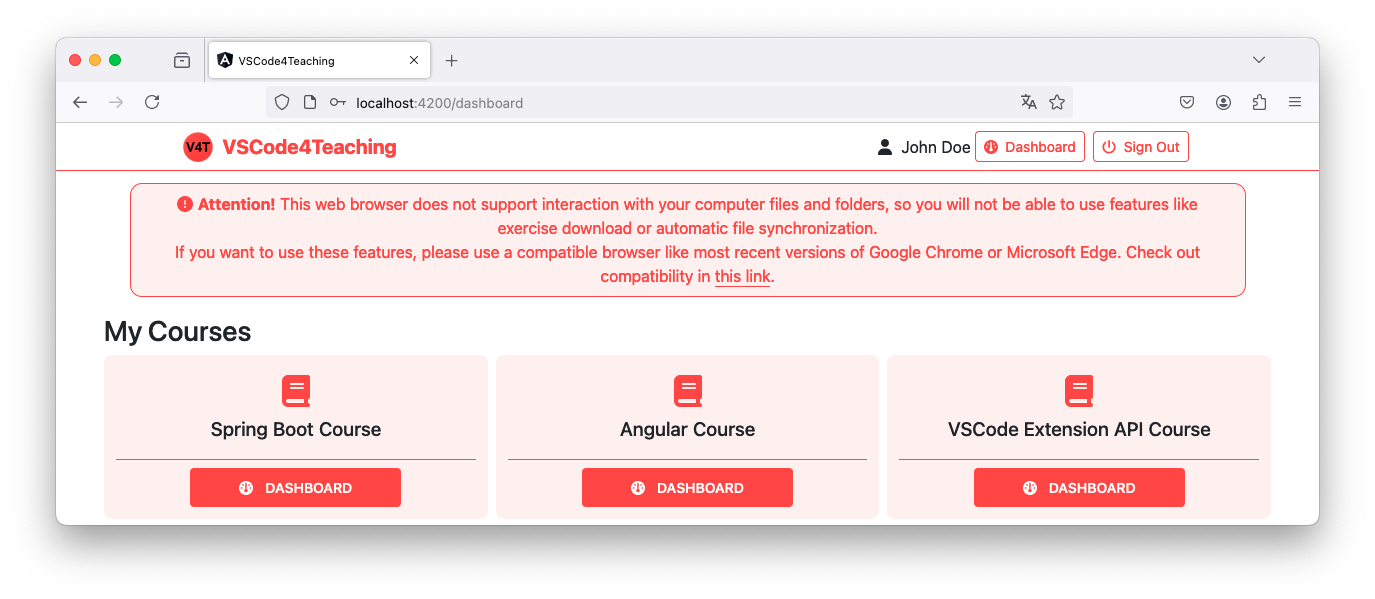
\includegraphics[width=\textwidth]{imagenes/utilizadas/4-3-implementacion/rn1-1.png}
    \caption{\textit{Dashboard} inicial de docentes en Firefox con aviso de incompatibilidad para el uso de la \textit{File System Access API}.}
    \label{fig:reqn1-1}
\end{figure}

\subsubsection{\texttt{RN-2}: aspecto visual de la aplicación web y coherencia entre interfaces}
\label{subsec:rn2}

El diseño de la interfaz de usuario de la nueva aplicación web aspira a ser coherente con la estética que venía empleándose en la extensión para Visual Studio Code, pretendiendo formar un entono familiar para quien ya utilizase la extensión de \textit{VSCode4Teaching} para Visual Studio Code.

La \referenciaFigura{fig:reqn2-1} muestra los dos \textit{dashboards} para el seguimiento del progreso de los ejercicios existentes: el de la extensión (abajo), que no se ha visto modificado y ya existía; y el de la aplicación web (arriba), que, inspirado en el diseño anterior, refleja la misma información haciendo uso de elementos gráficos de similar índole, ya que emplea el mismo esquema cromático y los mismos iconos informativos.

Esto también se observa en la \referenciaFigura{fig:reqn2-2}, que permite observar que los iconos empleados para la distinción de las tipologías de ejercicios son los mismos y que los dispuestos para las acciones de gestión de matriculados, compartición y adición de ejercicios son muy similares, potenciando la familiaridad del entorno a los usuarios.

\begin{figure}[!p]
    \centering
    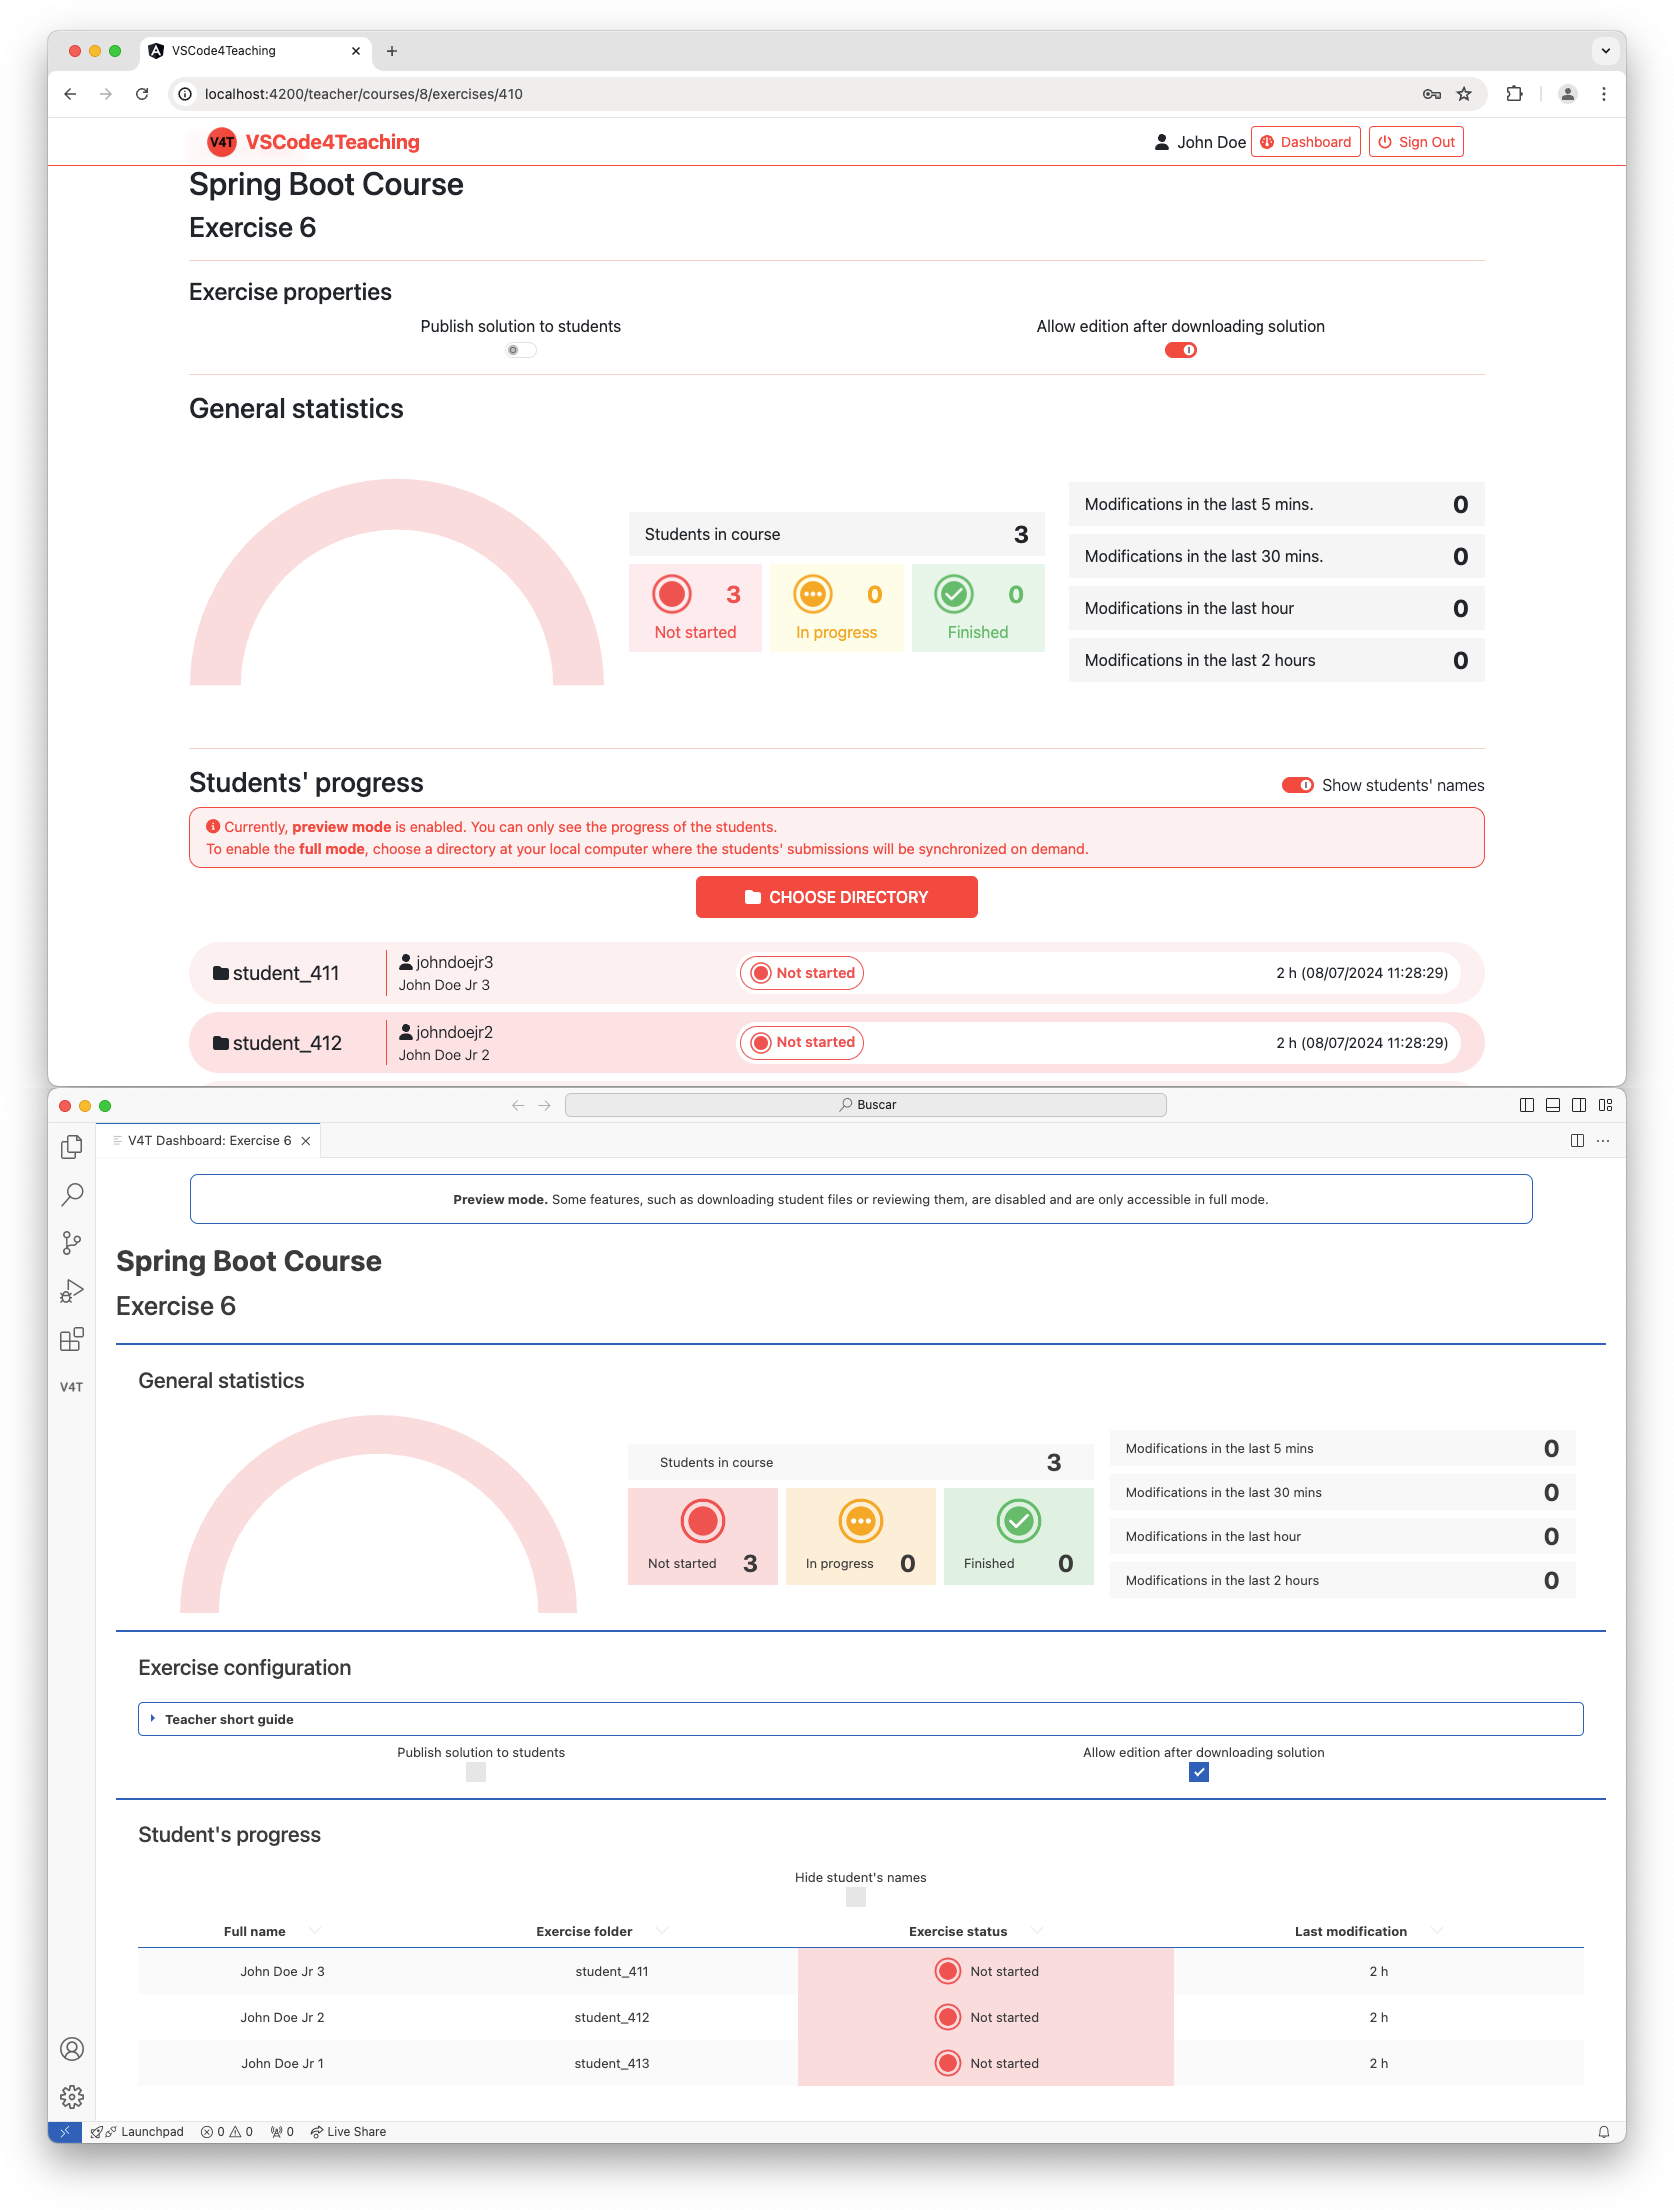
\includegraphics[width=\textwidth]{imagenes/utilizadas/4-3-implementacion/rn2-1.png}
    \caption{\textit{Dashboard} de un mismo ejercicio capturados a la vez en la aplicación web (arriba) y en la extensión para Visual Studio Code (abajo).}
    \label{fig:reqn2-1}
\end{figure}

\begin{figure}[ht!]
    \centering
    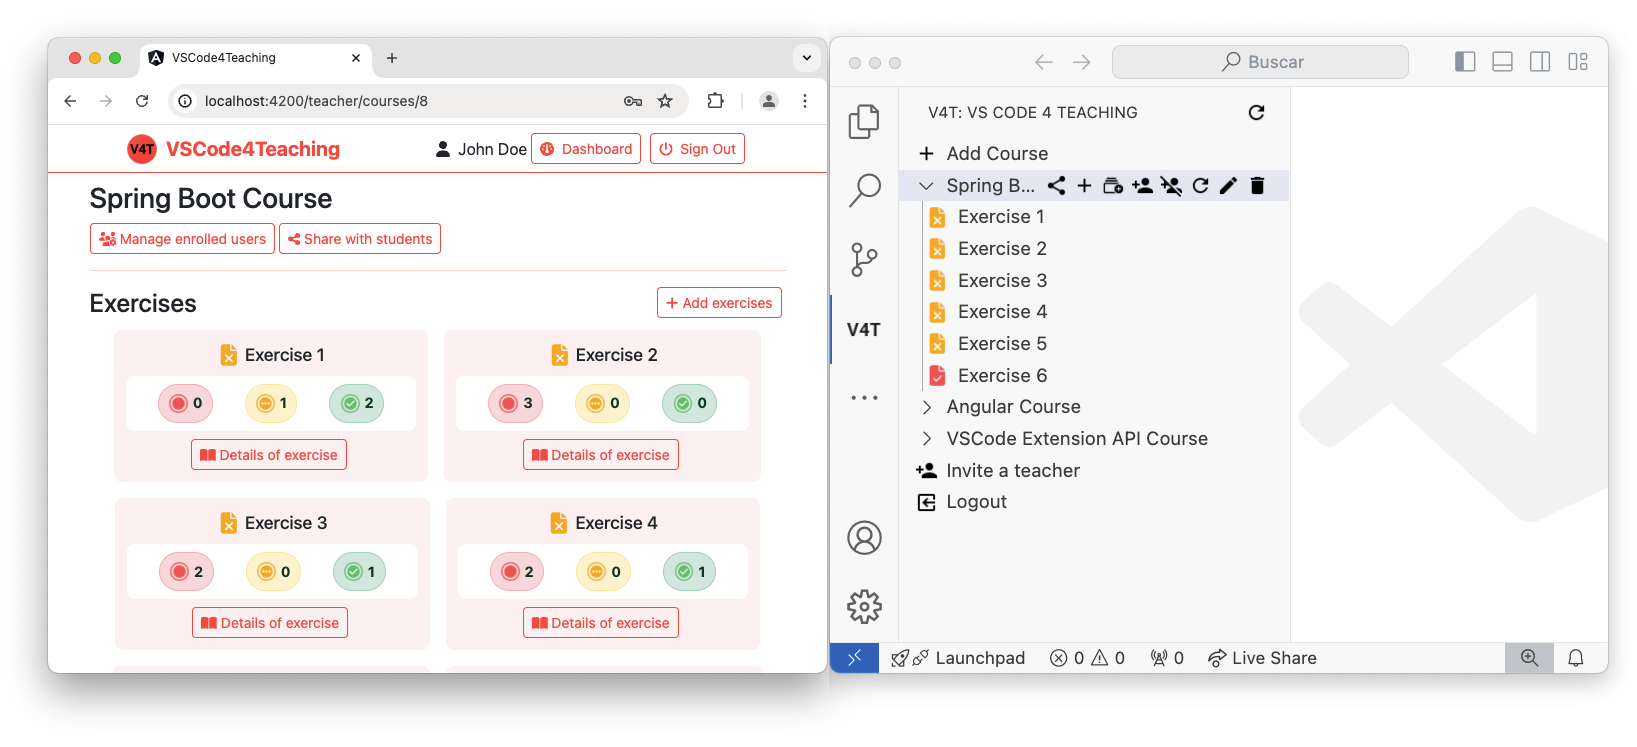
\includegraphics[width=\textwidth]{imagenes/utilizadas/4-3-implementacion/rn2-2.png}
    \caption{Comparativa entre los formatos empleados para mostrar a los docentes los ejercicios y configuraciones de las que disponen sus cursos.}
    \label{fig:reqn2-2}
\end{figure}

\subsubsection{\texttt{RN-3}: encriptación de \textit{tokens} JWT para autenticación}
\label{subsec:rn3}

El servidor de \textit{VSCode4Teaching} es \textit{stateless}; es decir, no almacena información sobre las interacciones realizadas por los usuarios con objeto de condicionar las siguientes, sino que cada una de las peticiones realizadas debe ser autocontenida e incluye en sí misma mediante sus cabeceras y cuerpo (si lo tiene) todo aquello que se debe tener en cuenta para proporcionar una respuesta, de modo que ninguna respuesta dependerá de las peticiones anteriormente realizadas \cite{Stateless}.

Si \textit{VSCode4Teaching} verifica esta característica es porque emplea \textit{tokens} JWT (siglas de \textit{JSON web token}, del inglés ``\textit{token} web en JSON'') para la autenticación de los usuarios. Estos \textit{tokens} son piezas de información representadas como cadenas de caracteres que permiten autenticar a los usuarios de forma autocontenida, ya que incluyen en sí mismos un \textit{payload} o carga útil que recoge qué usuario es el que está realizando una determinada petición. Se generan durante el inicio de sesión y quedan firmados mediante una clave privada, por lo que la suplantación de un usuario mediante un \textit{token} distinto del expedido durante la autenticación es inviable.

Sobre este mecanismo de autenticación preexistente, el presente requisito implementa el soporte a \textit{tokens} que, una vez generados, son encriptados nuevamente mediante un cifrado simétrico para añadir una capa adicional de seguridad. Este nuevo cifrado permite obtener cadenas no directamente comprensibles como \textit{tokens} JWT, añadiendo al servidor la lógica necesaria para manejar la presencia de cabeceras personalizadas llamadas \texttt{Encrypted-Authorization} en las peticiones procedentes de la aplicación web mediante la API REST y, además, como parámetro en la llamada inicial de las conexiones mediante \textit{Web Socket}.

\subsubsection{\texttt{RN-4}: adaptación de generación de imágenes Docker a nueva arquitectura}
\label{subsec:rn4}

El proyecto \textit{VSCode4Teaching} ya contaba previamente con la capacidad ejecutar su servidor a través de una imagen Docker, embebiendo en él la aplicación web Angular auxiliar como recurso estático. Además, se disponía de un fichero en formato YAML\footnote{YAML. Siglas de ``otro lenguaje de marcado más'' (del inglés \textit{Yet Another Markup Language}). Es un lenguaje de marcado de fácil lectura y comprensión que se aprovecha de la indentación para la jerarquización de declaraciones.}, \textit{docker-compose.yml}, para la orquestación de esta imagen con un contenedor para el sistema de persistencia basado en MySQL mediante Docker Compose.

Aunque la arquitectura del proyecto no ha variado al ejecutar la evolución realizada en este Trabajo Fin de Grado, se confiere mayor importancia a la aplicación web, que ahora busca ser sustitutiva o complementaria a la extensión para Visual Studio Code. La aplicación web auxiliar empleada anteriormente quedaba desplegada en el servidor en la ruta \texttt{/app}. Para mostrarla directamente al acceder a la raíz y, además, hacerla completamente compatible con el sistema de \textit{routing} propio de Angular (más información en la \referenciaSeccion{subsec:tecAngular}), se ha modificado el formato del despliegue e introducido un nuevo interceptor en el servidor que actúa como \textit{middleware}; esto es, como una capa intermedia de lógica ejecutada antes que el cotejamiento de rutas del servidor que tiene como finalidad detectar si las peticiones entrantes deben ser respondidas por el propio servidor o si deben ser derivadas a la aplicación web Angular para que esta, a través de su propia lógica de enrutamiento, ofrezca como respuesta los recursos gráficos necesarios.

Esta modificación de la lógica ha permitido preservar el método previamente empleado para la generación de la imagen Docker del servidor y la aplicación web. Esta configuración está alojada en el fichero \textit{Dockerfile} situado en la raíz del proyecto, en el que se define la construcción de la imagen en formato \textit{multi-stage}\footnote{\textit{Multi-stage}. Del inglés ``múltiples etapas'', se dice que un fichero de configuración es \textit{multi-stage} cuando se ejecutan varias fases en contenedores aislados y diferentes para dar lugar a una imagen final \cite{DockerfileMultistage}.}, articulándola en tres pasos ejecutados secuencialmente, tal como evidencia el \referenciaCodigo{cod:dockerfile}: compilación de la aplicación Angular en un contenedor Node, dando lugar a sendos recursos estáticos, compilación del servidor en un contenedor Maven (junto con los ficheros estáticos obtenidos en el paso anterior, que quedan copiados dentro del directorio del servidor destinado a este tipo de recursos) y generación de la imagen final sobre una base JDK que permite ejecutar la aplicación Java compilada en el paso anterior.

\begin{lstlisting}[language=Dockerfile,caption={Fichero \textit{Dockerfile} del proyecto, encargado de definir el proceso de generación de la imagen Docker del servidor y la aplicación web.},label=cod:dockerfile]
FROM node:18 AS angular
COPY vscode4teaching-webapp /usr/src/app
WORKDIR /usr/src/app
RUN ["npm", "install"]
RUN ["npm", "run", "build"]

FROM maven:3.9.7-eclipse-temurin-11 AS builder
COPY vscode4teaching-server /data
COPY --from=angular /usr/src/app/dist/vscode4teaching /data/src/main/resources/static/
WORKDIR /data
RUN ["mvn", "clean", "package"]

FROM eclipse-temurin:11
COPY --from=builder /data/target/vscode4teaching-server-*.jar ./app/vscode4teaching-server.jar
EXPOSE 8080
ENTRYPOINT [ "java", "-jar", "./app/vscode4teaching-server.jar" ]
\end{lstlisting}

Además, se ha ejecutado un cambio de localización de ficheros: la definición de Docker Compose, \textit{docker-compose.yml}, y el que contiene las variables de entorno que este último emplea (\textit{.env}) se han trasladado a la raíz del proyecto, donde ya se localizaba previamente el \textit{Dockerfile}.

Anteriormente se introducía en la imagen Docker un \textit{script} de \textit{shell} para organizar la sincronización de dependencias: preguntaba cada cierto tiempo si se disponía de una conexión válida con el sistema de persistencia configurado y solo cuando esta condición se cumplía, el \textit{script} lanzaba la ejecución del servidor, que requiere necesariamente disponer de la base de datos configurada desde su mismo inicio. Esta implementación se ha visto reemplazada por el uso del mecanismo de \textit{healthcheck}, que es una comprobación declarada como parte de la imagen empleada para la ejecución del contenedor de la base de datos, de modo que se relega en Docker Compose la responsabilidad de orquestar el funcionamiento de ambos contenedores. El \referenciaCodigo{cod:dockerCompose} muestra un fragmento del fichero \textit{docker-compose.yml} en el que se configura la dependencia entre contenedores y el mecanismo de espera mediante esta comprobación: la aplicación declara ser dependiente de la base de datos (\texttt{depends-on}), por lo que Docker Compose no ejecutará este contenedor hasta que la base de datos esté ``sana'', introduciendo en su configuración el mecanismo para comprobar cuándo este contenedor alcanza esta condición tras su inicialización.

\begin{lstlisting}[language=YAML,caption={Fichero \textit{docker-compose.yml} empleado para la orquestación de la imagen Docker del servidor con un contenedor para la base de datos.},label=cod:dockerCompose]
name: vscode4teaching

services:
  app:
    image: vscode4teaching/vscode4teaching:latest
    depends_on:
      db:
        condition: service_healthy
    env_file:
      - path: .env
        required: true
    ports:
      - ${SERVER_PORT}:${SERVER_PORT}
    volumes:
      - ./volume-v4t:${V4T_FILEDIRECTORY}
    restart: on-failure:6
  db:
    image: mysql:8.4.0
    restart: on-failure:3
    environment:
      MYSQL_ROOT_PASSWORD: ${MYSQL_ROOT_PASSWORD}
      MYSQL_DATABASE: ${MYSQL_DATABASE}
      MYSQL_USER: ${SPRING_DATASOURCE_USERNAME}
      MYSQL_PASSWORD: ${SPRING_DATASOURCE_PASSWORD}
    volumes:
      - ./volume-mysql:/var/lib/mysql
    healthcheck:
      test: "mysqladmin ping -h 127.0.0.1 || exit 1"
      interval: 5s
      timeout: 5s
      retries: 5
\end{lstlisting}

\subsubsection{\texttt{RN-5}: migración a GitHub Actions del sistema de integración continua}
\label{subsec:rn5}

Previamente al inicio del presente Trabajo Fin de Grado, el proyecto \textit{VSCode4Teaching} hacía uso de un sistema de integración y despliegue continuos a través de \textbf{Travis CI} en el que recaían tres tareas: cada vez que se producían modificaciones en la rama \texttt{master}, se ejecutaban las pruebas automáticas de servidor y extensión y, además, se publicaban nuevas etiquetas de la imagen del servidor en el repositorio en Docker Hub.

Este sistema se ha visto reemplazado por GitHub Actions, descrito en la \referenciaSeccion{subsec:herCiCd}. Sin embargo, esta migración no se ha limitado a replicar la funcionalidad previamente utilizada en el sistema de integración, entrega y despliegue continuos sino que, además, se ha aprovechado para ampliar su alcance.

Como consecuencia, el proyecto \textit{software} de \textit{VSCode4Teaching} cuenta ahora con dos flujos de trabajo (\textit{workflows}) diferenciados por componentes. El primero de estos, dedicado a las tareas relativas al servidor y la aplicación web, cuenta con tres trabajos definidos:
\begin{itemize}
    \item \texttt{Test}. Es el trabajo encargado de la ejecución de la batería de pruebas automáticas implementada en el servidor. Se ejecuta cada vez que se produce una alteración en las ramas \texttt{master} o \texttt{develop} del proyecto y, además, cuando se produce un \textit{pull request}\footnote{\textit{Pull request}. En su origen, solicitud realizada al propietario legítimo de un código para realizar una incorporación de otro código implementado fuera del repositorio original. Actualmente, además, se utiliza como sistema organizativo que permite coordinar la fusión de las distintas ramas de un repositorio y dotar a este proceso de un entorno que permite debates entre programadores, solicitar aprobaciones y ejecutar validaciones automáticas, entre otros.} entre ellas para conocer el estado de las pruebas antes de fusionar cambios a la rama del código de producción.
    \item \texttt{Publish}. Se encarga de la publicación de las nuevas versiones lanzadas al repositorio en Docker Hub y, por tanto, se ejecuta cada vez que se modifica la rama \texttt{master}. Genera una imagen Docker utilizando la declaración existente en el proyecto (véase la \referenciaSeccion{subsec:rn4}) y la publica en el repositorio del proyecto en Docker Hub, liberando dos etiquetas: actualiza la versión \textit{latest} de la imagen y, además, genera una nueva específica para la versión liberada.
    \item \texttt{Deploy}. Una vez publicada una nueva versión en Docker Hub, se accede mediante SSH\footnote{SSH. Siglas de ``terminal seguro'' (del inglés \textit{Secure SHell}). Es un protocolo utilizado para la administración remota de computadores.} a la máquina de producción, le transfiere una nueva versión del fichero Docker Compose en la que se utiliza la nueva versión puesta en producción, descarga la imagen desde Docker Hub y aplica los cambios al despliegue, dejando activa en producción la nueva versión automáticamente.
\end{itemize}

Análogamente, se declara un flujo de trabajo para la extensión que comprende únicamente los dos primeros trabajos descritos para el caso anterior, particularizándolos para la plataforma \textit{software} que emplea este componente. De este modo, para la extensión se ejecuta la batería de pruebas automáticas tras cada \textit{commit} en las ramas \texttt{master}, \texttt{develop} y cuando se produzca un \textit{pull request} entre ellas y, si se ha lanzado una nueva versión, se publica automáticamente en el Visual Studio Code Marketplace.

Todos los flujos anteriormente descritos quedan declarados en sendos ficheros YAML dentro del directorio \texttt{.github/workflows} en el proyecto, siendo esta la ubicación requerida por GitHub Actions para ejecutarlos automáticamente. Sirva como ejemplo el \referenciaCodigo{cod:ciGitHubTestServer}, que es la especificación para GitHub Actions del trabajo que ejecuta las pruebas automáticas del servidor, que es el primero de los especificados en el fichero \texttt{server.ci.yml}.

\begin{lstlisting}[language=YAML,caption={Fragmento del flujo de trabajo de acciones automáticas relativas a la integración continua del servidor.},label=cod:ciGitHubTestServer]
name: "Server pipeline"

on:
  push:
    branches:
      - master
      - main
      - develop
  pull_request:
    branches:
      - master
      - main
      - develop

jobs:
  test:
    runs-on: ubuntu-latest
    defaults:
      run:
        working-directory: ./vscode4teaching-server
    steps:
      - name: Checkout repository
        uses: actions/checkout@v4
      - name: Set up Java version
        uses: actions/setup-java@v4
        with:
          java-version: 11
          distribution: temurin
      - name: Test
        run: ./mvnw clean dependency:resolve test
  publish:
    if: ${{ github.event_name == 'push' && github.ref == 'refs/heads/main' }}
    needs: test
    # [...]   
  deploy:
    if: ${{ github.event_name == 'push' && github.ref == 'refs/heads/main' }}
    needs: publish
    # [...]
\end{lstlisting}

En la \referenciaFigura{fig:reqn5-1} se muestra una parte del histórico de ejecuciones de los flujos de trabajo definidos para varios \textit{commits} ejecutados sobre la rama \texttt{develop}. GitHub Actions posibilita acceder al detalle de cada ejecución, permitiendo visualizar gráficamente el estado y disposición de los trabajos realizados. Además, en caso de ser necesario, también se pueden obtener los registros en detalle de la ejecución de cada uno de los trabajos que componen un flujo.

\begin{figure}[h]
    \centering
    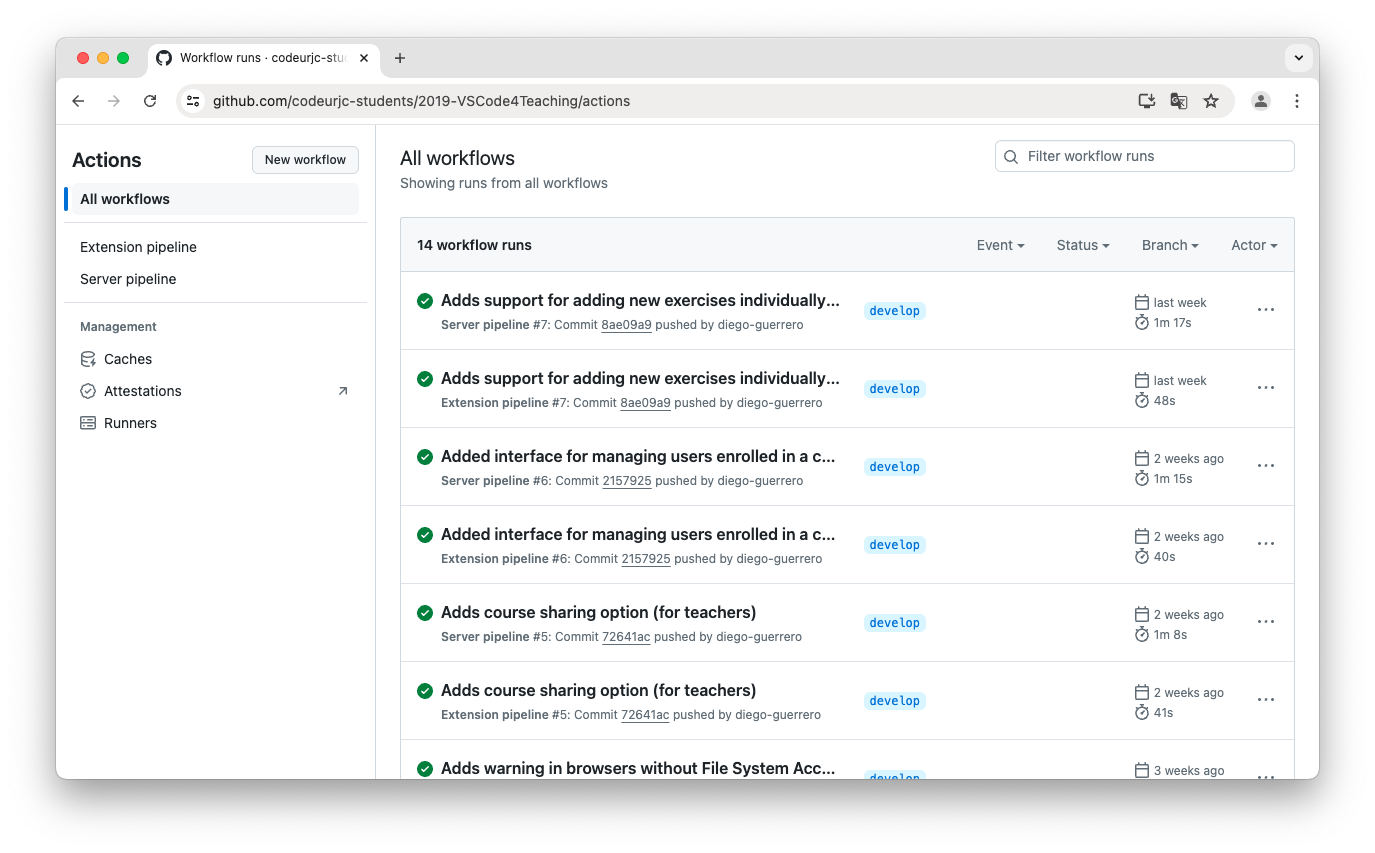
\includegraphics[width=\textwidth]{imagenes/utilizadas/4-3-implementacion/rn5-1.png}
    \caption{Fragmento del listado de ejecuciones de los flujos de trabajo de integración continua con GitHub Actions.}
    \label{fig:reqn5-1}
\end{figure}



% Sección 4.4: Pruebas
%  En esta sección se describen las pruebas automáticas que han sido implementadas para el proyecto. Sobre los tests,
%  conviene indicar la cobertura del código. Si no se han implementado pruebas automáticas, deberían haberse
%  implementado y describirse aquí o tener una buena justificación de por qué no se han implementado.
\section{Verificación de \textit{software} y funcionalidad}
\label{sec:verificacion}
Muchos teóricos de la ingeniería del \textit{software} afirman que la verificación del código mediante pruebas es indispensable para poder garantizar su calidad. Por ejemplo, Robert C. Martin afirma que ``las pruebas unitarias son necesarias para garantizar que el código es flexible, mantenible y reutilizable, ya que eliminan el miedo a hacer modificaciones en el código'' \cite{CleanCode}.

La nueva aplicación web implementada durante el presente hito evolutivo de \textit{VSCode4Teaching} no incluye pruebas automáticas, ya que se ha primado alcanzar una versión funcional de la aplicación por encima de la verificación de su comportamiento, que requerirá de la implementación de pruebas de tres tipos: unitarias, para corroborar el funcionamiento de la lógica de negocio; de integración, para la comprobación de la correcta comunicación con el servidor; y \textit{end-to-end} o de interfaz, con el fin de verificar que la interfaz de usuario se adecía a los requerimientos específicos de cada situación; pudiendo verse complementadas por otros tipos de pruebas, como las de carga o rendimiento, las de accesibilidad o las pruebas de funcionamiento en múltiples navegadores, especialmente importantes en este caso por las divergencias de compatibilidad de las tecnologías empleadas. La incorporación de pruebas automáticas para la garantía de la calidad de la aplicación web es uno de los primeros trabajos a futuro del proyecto, tal como recoge la \referenciaSeccion{subsec:trabajosFuturos}.

El servidor y la extensión cuentan con pruebas automáticas implementadas. Estas pruebas se basan en el uso de aserciones, que son comparaciones entre los valores obtenidos al ejecutar las pruebas y los valores deseados; y en dobles, que son piezas \textit{software} que permiten sustituir las dependencias empleadas que queden fuera del ámbito de la prueba realizada para simular su comportamiento en un escenario real y poder ejecutar la prueba al completo proporcionando valores conocidos a la salida de la dependencia reemplazada.

Las pruebas implementadas son de dos tipos: unitarias, que son aquellas que tienen como alcance una sola capa del \textit{software} y que emplean dobles para simular el funcionamiento de sus dependencias; y de integración, que verifican cómo interactúan entre sí las distintas capas del mismo componente o cómo se produce la comunicación entre el componente verificado y otros agentes \textit{software}.

\subsection{Pruebas automáticas del servidor}
\label{subsec:testingServidor}
Tal como consta en la \referenciaSeccion{subsec:tecServidor}, el servidor hace uso de JUnit para la implementación y ejecución de las pruebas automáticas implementadas en el servidor. Esta biblioteca incorpora una amplia cantidad de aserciones y permite generar dobles de dependencias de forma sencilla para el implementador. El servidor incluye \textit{tests} de tres tipos:
\begin{itemize}
    \item Pruebas sobre controladores. Incluidas en el paquete \texttt{controllertests}, son pruebas unitarias que verifican el correcto funcionamiento de la capa de los controladores REST de Spring y que se implementan ejecutando llamadas HTTP a la aplicación y utilizando dobles que suplantan el funcionamiento de los servicios que emplean para la generación de la respuesta.
    \item Pruebas sobre servicios. Localizadas en el paquete \texttt{servicetests}, son pruebas unitarias que buscan verificar el correcto funcionamiento de la capa de los servicios Spring, que es la que incluye la traslación al \textit{software} de la lógica de negocio, y se implementan mediante la suplantación con dobles de los DAO de la aplicación, proporcionando instancias basadas en un conjunto de valores conocidos.
    \item Pruebas de integración. Ubicadas en el paquete \texttt{integrationtests}, y al contrario que las anteriores, son pruebas que verifican el funcionamiento de la aplicación en su integridad, lanzando una petición HTTP y sin proporcionar ningún tipo de doble. Emplean un mecanismo para la inicialización de valores conocidos en una base de datos embebida en la aplicación e instanciada únicamente durante el lanzamiento de estas pruebas, hecho que posibilita la ejecución de pruebas que validan la correcta interacción entre las capas de la arquitectura y, además, con el sistema de persistencia.
\end{itemize}

Cuantitativamente, la batería de pruebas automáticas del servidor contiene un total de 96 pruebas que alcanzan un $78,3\%$ de las clases y un $79,4\%$ de los métodos que conforman este componente.

\subsection{Pruebas automáticas de la extensión}
\label{subsec:testingExtension}
Análogamente al caso anterior, y tal como enuncia la \referenciaSeccion{subsec:tecExtension}, la extensión para Visual Studio Code también incluye una batería de pruebas automáticas implementada sobre Jest que permite verificar el correcto funcionamiento de este componente en su integridad.

Las pruebas incorporadas a la extensión permiten verificar el correcto funcionamiento de su arquitectura en su práctica totalidad, para lo que incorpora 129 pruebas automáticas. Entre ellas, cabe reseñar una cobertura del código superior al $80\%$ sobre el cliente empleado para el intercambio de peticiones con el servidor, sobre algunos de los elementos empleados en la interfaz de usuario (como los elementos mostrados en la barra de actividad) y sobre el modelo del dominio. El dato de cobertura total de la extensión es de un $61,7\%$ de las líneas de código del proyecto y de un $54,9\%$ de las funciones que incorpora.


% Sección 4.5: Distribución y despliegue
\section{Distribución}
\label{sec:distribucion}
Se introduce a continuación la forma en que se divulga el proyecto \textit{VSCode4Teaching} en sus distintas etapas: tanto como código fuente (\referenciaSeccion{subsec:distribFuente}) como los artefactos construidos de la extensión y el servidor con la aplicación web (\referenciaSeccion{subsec:distribArtefactos}).

\subsection{Distribución del código fuente}
\label{subsec:distribFuente}
El código fuente del proyecto \textit{VSCode4Teaching} se encuentra íntegramente publicado en la red a través de un repositorio alojado en GitHub (\referenciaSeccion{subsec:tecGitHub}), tal como ilustra la \referenciaFigura{fig:distribGitHub}.

\begin{figure}[ht]
    \centering
    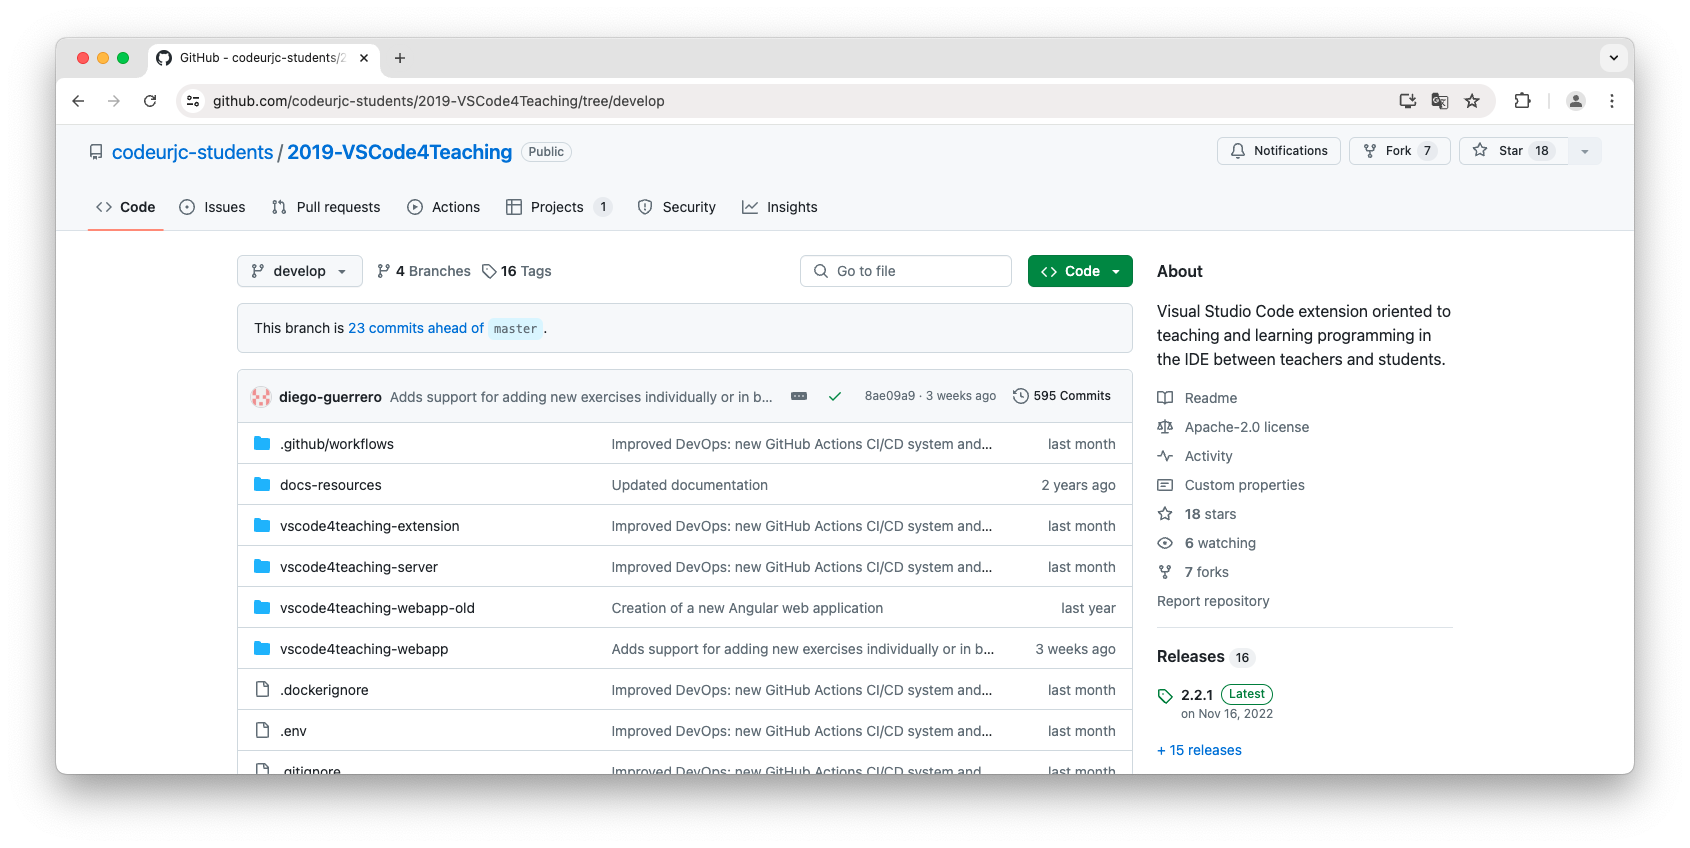
\includegraphics[width=0.8\linewidth]{imagenes/utilizadas/4-5-distribucion/repoGitHub.png}
    \caption{Repositorio en GitHub del proyecto \textit{VSCode4Teaching}.}
    \label{fig:distribGitHub}
\end{figure}

Este repositorio viene utilizándose desde el inicio del proyecto y contiene el histórico completo de cambios producidos en la aplicación durante su evolución. Se encuentra alojado en la siguiente dirección:

\vspace{-0.7\baselineskip}
\begin{center}
    \href{https://github.com/codeurjc-students/2019-VSCode4Teaching}{https://github.com/codeurjc-students/2019-VSCode4Teaching}.
\end{center}
\vspace{-0.7\baselineskip}

Tal como incluye en el fichero \texttt{LICENSE} alojado en su raíz, el código fuente de \textit{VSCode4Teaching} está sujeto a la licencia Apache License 2.0 \cite{ApacheLicense}. Esta licencia es permisiva y permite a otros desarrolladores utilizar el código del proyecto para su modificación y redistribución libremente siempre y cuando se mantenga la licencia sobre todas aquellas partes del fuente que no hayan sido adaptadas en las nuevas versiones generadas.

Esta licencia permite, además, aseverar que \textit{VSCode4Teaching} es \textit{software} libre, ya que otorga a sus usuarios las cuatro libertades esenciales: libertad de ejecutarlo como se desee y para lo que se desee, libertad de estudiar cómo funciona y poder adaptarlo para modificar su comportamiento, libertad para redistribuirlo y libertad para distribuir también las copias modificadas \cite{FreeSoftwareFreedoms}.

\subsection{Distribución de artefactos}
\label{subsec:distribArtefactos}
Además de la distribución de su código fuente, el proyecto \textit{VSCode4Teaching} publica sus artefactos empaquetados para una utilización directa más sencilla de la aplicación. Tal como se introduce en la \referenciaSeccion{subsec:tecDistrib}, se hace uso de dos repositorios públicos para la divulgación de la extensión para Visual Studio Code y del servidor empaquetado junto con la aplicación web en una imagen Docker (véase el requisito \referenciaConTT{subsec:rn4}{RN-4}).

La extensión queda publicada mediante el sistema de integración continua (véase el requisito \referenciaConTT{subsec:rn5}{RN-5}) en el Visual Studio Code Marketplace, lo que posibilita que esté disponible directamente para los usuarios a través de la herramienta integrada para la búsqueda e instalación de extensiones, tal como muestra la \referenciaFigura{fig:distribVSCodeMarketplace}.
\begin{figure}[ht]
    \centering
    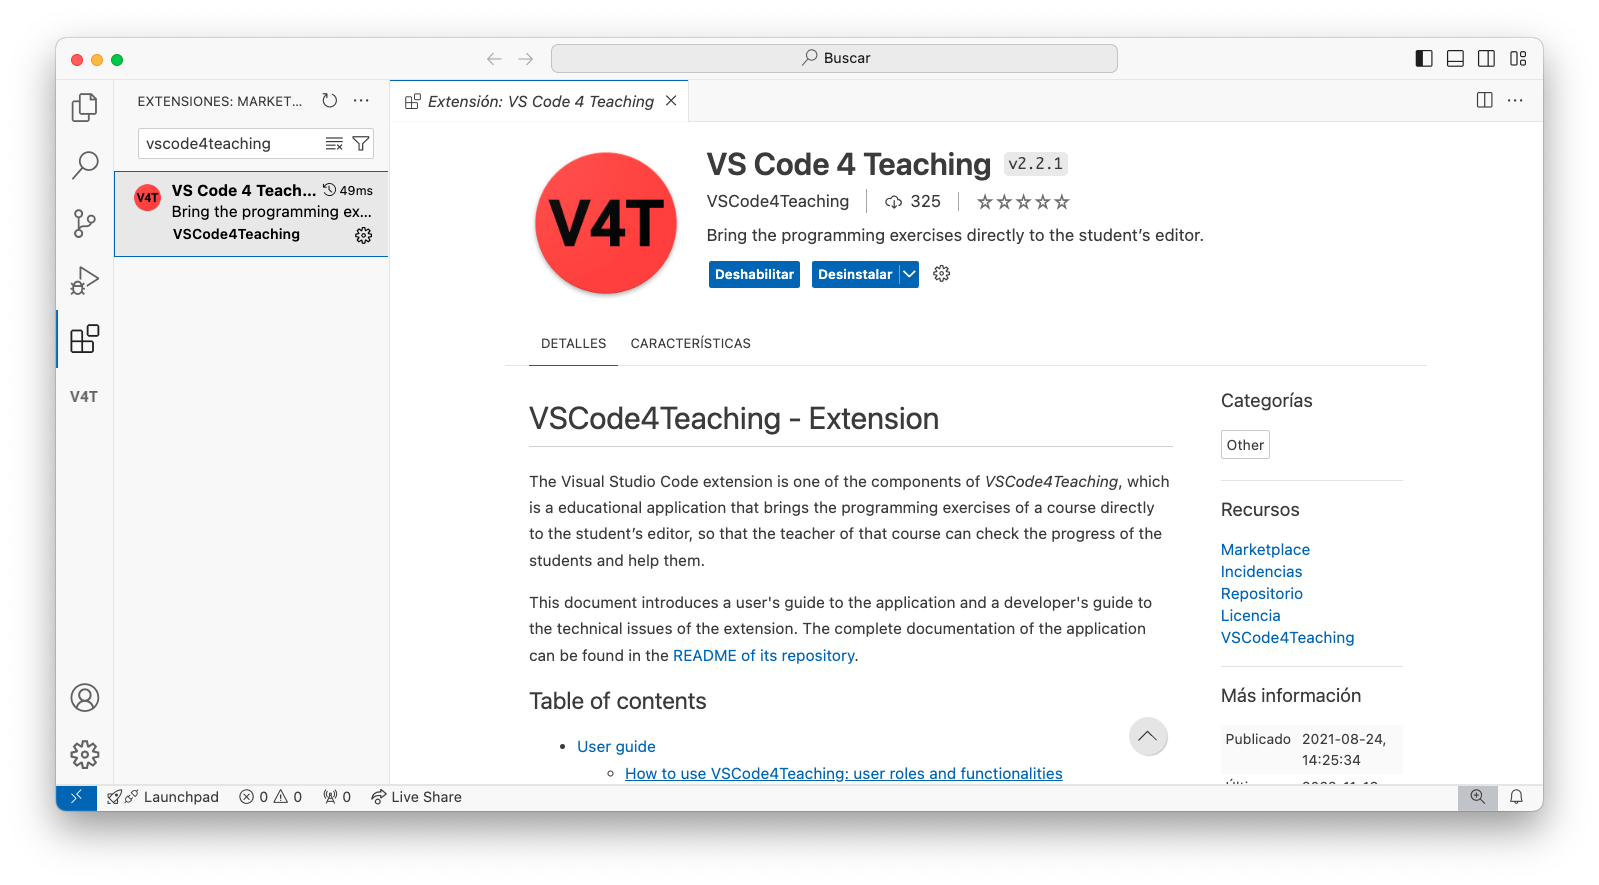
\includegraphics[width=0.8\linewidth]{imagenes/utilizadas/4-5-distribucion/vscodeMarketplace.png}
    \caption{Extensión de \textit{VSCode4Teaching} en el área de búsqueda y descarga de extensiones en Visual Studio Code.}
    \label{fig:distribVSCodeMarketplace}
\end{figure}

\noindent El enlace a la extensión publicada es el siguiente:
\vspace{-0.7\baselineskip}
\begin{center}
    \href{https://marketplace.visualstudio.com/items?itemName=VSCode4Teaching.vscode4teaching}{https://marketplace.visualstudio.com/items\\ ?itemName=VSCode4Teaching.vscode4teaching}.
\end{center}
\vspace{-0.7\baselineskip}

Por otro lado, el servidor queda empaquetado junto con la aplicación web como \textit{frontend} en una imagen Docker generada mediante el sistema de CI/CD que queda publicada en el Docker Hub, tal como se detalla en los requisitos \referenciaConTT{subsec:rn4}{RN-4} (acerca de la generación) y \referenciaConTT{subsec:rn5}{RN-5} (sobre la automatización), quedando disponible para su utilización mediante, por ejemplo, el fichero \textit{docker-compose.yml} disponible en el repositorio.

\noindent El enlace a la imagen publicada del servidor con la aplicación web es el siguiente:
\vspace{-0.7\baselineskip}
\begin{center}
    \href{https://hub.docker.com/r/vscode4teaching/vscode4teaching}{https://hub.docker.com/r/vscode4teaching/vscode4teaching}.
\end{center}
\vspace{-0.7\baselineskip}

